%%%%%%%%%%%%%%%%%%%%%% Version Information %%%%%%%%%%%%%%%%%%%%%%%%%%% 
% This LaTeX2e thesis template is based on the nuthesis-template
% provided by Miguel A. Lerma. It was renamed and edited to meet the
% requirements given in the Thesis-Dissertation Instructions of the
% School of Graduate Studies of Case Western Reserve University by
% Initial Version: Frank Ernst (Dr. rer. nat. habil., Professor). 
%   Version dated 2006-08-23.
% Latest Version: Roger French (Professor). 
%  SDLE Center Authors: Nicholas Wheeler, Myles Murray, Heather Lemire
%  Version dated 2015
%%%%%%%%%%%%%%%%%%%%%%%%%%%%%%%%%%%%%%%%%%%%%%%%%%%%%%%%%%%%%%%%%%%%%% 

%%%%%%%%%%%%%%%%%%%%%%%%%%%%%% DISCLAIMER %%%%%%%%%%%%%%%%%%%%%%%%%%%%
% The author of the thesis remains responsible for fulfilling all
% requirements.
%%%%%%%%%%%%%%%%%%%%%%%%%%%%%%%%%%%%%%%%%%%%%%%%%%%%%%%%%%%%%%%%%%%%%%

%%%%%%%%%%%%%%%%%%%%%%%%%%%%% DESCRIPTION %%%%%%%%%%%%%%%%%%%%%%%%%%%%
% cwru-cse-thesis.tex is the master file that compiles the whole thesis.
% Individual chapter files located in 'content' folder
% Appendix files located in 'app' folder
% bibtex file for references located in 'refs' folder
% figure files go in the 'figs' folder
% the 'input' folder has style files for tex compiling
%%%%%%%%%%%%%%%%%%%%%%%%%%%%%%%%%%%%%%%%%%%%%%%%%%%%%%%%%%%%%%%%%%%%%%

\documentclass[help,12pt,onepage,reqno]{input/CWRU-Thesis}



%%%%%%%%%%%%%
% EQUATIONS %
%%%%%%%%%%%%%

% ArgMin
\DeclareMathOperator*{\argmin}{\arg\!\min}

% ArgMax
\DeclareMathOperator*{\argmax}{\arg\!\max}

%%%%%%%%%%%%%%%%%%%%%%%%%%%%%%%%%%%%%%%%%%%%%%%%%%%%%%%%%%%%%%%%%%%%%%%%%%%%%%%%%%%%%%%%%%%%%%%%%%%%



% Uncomment *one* of the following lines if you are tired of TeX's
% Computer Modern fonts:
\usepackage{fourier} 
%\usepackage{mathpazo}
%\usepackage{mathptmx}

% Graphics.
\usepackage[pdftex]{graphicx}
\usepackage{subfig}
\usepackage{pdflscape} % landscape environment
%\usepackage{subfigure}
\usepackage{longtable}

% The following makes graphicx work with pdf and jpg files. Files with
% same names and different extensions will be recognized in sequential
% order.
\DeclareGraphicsExtensions{.png, .jpg, .pdf} 

% PDFPages imports entire PDF pages.
%\usepackage[draft]{pdfpages} % not sure that this actually works
\usepackage[final]{pdfpages}

% Sets pdftex to included versions up to 1.6
%\pdfminorversion=6
\pdfoptionpdfminorversion=6

% Chapterbib enables separate bibliographies after each chapter.
%\usepackage[sectionbib]{chapterbib}
%\usepackage[rootbib]{chapterbib}

\usepackage{verbatim} %for comment environment

% % to allow underscore in text, doesn't work if you actually use
% % underscores in the latex doc
% \usepackage{underscore}
% \begingroup
%   \lccode`\~=`\_
% \lowercase{\endgroup
%   \pdfstringdefDisableCommands{\let~\relax}%
% }

% Wrapfig wraps tables and figures.
\usepackage{wrapfig} 
\usepackage{multirow}

% footnotes in tables
\usepackage{threeparttable}
% \usepackage{footnote}
% \makesavenoteenv{tabular} % makes tables handle footnotes correctly

% Your packages can go here:
\usepackage{input/KL-Typing-Aids}

\usepackage{xcolor}
\usepackage{listings}
\lstset{basicstyle=\ttfamily,
  showstringspaces=false,
  commentstyle=\color{red},
  keywordstyle=\color{blue}
}


%%%%%%%%%%%%%%%%%%%%%%%%%%%%%%%%%%%%%%%%%%%%%%%%%%%%%%%%%%%%%%%%%%%%%%%%
% Author and title
\author{\uppercase{Peng Xu}}
\title{Adaptive Cruise Control with Deep Q Learning}

\degree{Master of Science}  
% Default: Doctor of Philosophy.

%\adviser{Dr. Roger H. French}     
% Optional -- Default: Empty.

\department{\deecs}     
% No Default.

\graduationmonth{May}      
% The default is January, May, or August depending on current date.

\graduationyear{2018}
% Default: current year.
% CAUTION: next January could be *next* year.


%\includeonly{05-Background, 06-Methods}
% Use \includeonly to select the chapters to include if you are using
% the \include command below. This way you can latex only a the part
% you are working on, which is faster than latexing the entire thesis.

% Margin kerning.
\input input/protcode.tex

%	%------------------- Markup
	% new commands for markup/editing purposes
	% make a \newcommand for your self, this rhf set is for Roger (rhf) and Dan (dmd)
	\usepackage{xcolor}
	\usepackage{ulem}
		% color names = red, green, blue, cyan, magenta, yellow, black, gray, white,  
		%   darkgray, lightgray, brown, lime, olive, orange, pink,  purple, teal, violet
		%   
			%-------------------------
				% rhf = Roger markup
			\newcommand{\rhf}{\textcolor{red}} % for rhf = Roger is red text
			\newcommand{\rhfcomm}[1]{
			       \colorbox{yellow}{#1} % Roger is yellow highlight
			       }
			\newcommand{\rhfstr}[1]{
				\sout{#1} %Roger's strikethrough
			}
			%-------------------------
			
\usepackage{hyperref} % enables hyper links in the document's pdf file output


%%%%%%%%%%%%%%%%%%%%%%%%%%%%%%%%%%%%%%%%%%%%%%%%%%%%%%%%%%%%%%%%%%%%%%%%
\begin{document}%%%%%%%%%%%%%%%%%%%%%%%%%%%%%%%%

%Margin kerning.
\setprotcode \font
{\it \setprotcode \font}
{\bf \setprotcode \font}
{\bf \it \setprotcode \font}

% % To turn off hyphen protrusion at end of line, set to "0".
\pdfprotrudechars=1 

\frontmatter
%\pagenumbering{roman}

% Title page.
\maketitle		

% Page for signatures of the committee members.
%For the final turn in, you do not need this page signed, just dated.
% to date this page, cludgy way to do it is replace Signature/Date with the Date
%Found in the CWRU-thesis.cls file, line 327
\signaturepage
\sign[Adviser]{Dr. Wyatt Newman}{Chair}{\deecs}
\sign{Dr. M. Cenk Cavusoglu}{Member}{\deecs}
%\sign{\fe}{Member}{\deecs} %if pre programed can use short name thing

% Copyright page. You do not need a copyright page unless
% you are applying for a copyright.
%\copyrightpage 

% Dedication page (optional). Please indicate linebreaks by "\\".
\dedication{Dedicated to *your\\dedication message goes here*}

% Preface (optional).
%\preface
%\input{03-Preface}

% Table of Contents will be automatically generated and placed here.
\tableofcontents

% List of Tables and List of Figures will be automatically generated
% and placed here.
\listoftables	
%\subfiglabelskip=0pt % suppresses spacing after empty subfiglabel set
                     % to 0pt; for use with subfigure.sty
\listoffigures		


%%%%%%%%%%%%%%%%%%%%%%%%%%%%%%%%%%%%%%%%%%%%%%%%%%%%%%%%%%%%%%%%%%%%%%%%
% Acknowledgements (optional).
\acknowledgements
\begin{sloppypar}
\section{Acknowledgements}


\end{sloppypar}


%%%%%%%%%%%%%%%%%%%%%%%%%%%%%%%%%%%%%%%%%%%%%%%%%%%%%%%%%%%%%%%%%%%%%%%%
% Abstracts must not exceed 350 words in dissertations and 150
% words in other theses.
\abstract
\begin{sloppypar}
\section{Abstract}


The present paper describes a study that aims at assessment of driver behavior in response to new technology, particularly Adaptive Cruise Control Systems (ACCs), as a function of driving style. In this study possible benefits and drawbacks of Adaptive Cruise Control Systems (ACCs) were assessed by having participants drive in a simulator. The four groups of participants taking part differed on reported driving styles concerning Speed (driving fast) and Focus (the ability to ignore distractions), and drove in ways which were consistent with these opinions. The results show behavioral adaptation with an ACC in terms of higher speed, smaller minimum time headway and larger brake force. Driving style group made little difference to these behavioral adaptations. Most drivers evaluated the ACC system very positively, but the undesirable behavioral adaptations observed should encourage caution about the potential safety of such systems.

\newpage
\end{sloppypar}
%can you run bibliography on abstract?
%\bibliographystyle{plainnat}
%\bibliography{my_references}
 

\mainmatter             
\pagenumbering{arabic} 

% Change hyperlink color to a bluish hue that is fairly visible, but
% not disturbing in long lists of references, and will also print well
% in black and white. Up to this point, the hyperlink color was black
% (default) to avoid that the tables of contents, figures, and tables
% entirely appear in color.
\definecolor{felinkcolor}{rgb}{0,0,0.5}


%%%%%%%%%%%%%%%%%%%%%%%%%%%%%%%%%%%%%%%%%%%%%%%%%%%%%%%%%%%%%%%%%%%%%%%%
\chapter{Introduction}


\section{Motivation and Background}

% Autonomous Vehicle

Modern technologies have the potential to create a paradigm shift in the vehicle-driver relationship with advanced automation changing the driver role from "driving" to "supervising". To design new driver environments that caters for these emerging technologies, traditional approaches identify current human and technical constraints to system efficiency and create solutions accordingly. However, there are two reasons why such approaches are limited within the technologically-evolving automotive domain. First, despite significant progress in the development of system theory and methods, the application of these methods is largely constrained to the existence of a current system. Second, there are few structured approaches for using the analysis results to support design. In this paper, an attempt is made to overcome these challenges by developing and implementing a method for analyzing and designing a highly autonomous commercial vehicle. 

An autonomous vehicle has great potential to improve driving safety, comfort and efficiency and can be widely applied in a variety of fields, such as road transportation, agriculture, planetary exploration, military purpose and so on \cite {WANG2015727}. The past three decades have witnessed the rapid development of autonomous vehicle technologies, which have attracted considerable interest and efforts from academia, industry, and governments. Particularly in the past decade, contributing to significant advances in sensing, computer technologies, and artificial intelligence, the autonomous vehicle has become an extraordinarily active research field. During this period, several well-known projects and competitions for autonomous vehicles have already exhibited autonomous vehicles' great potentials in the areas ranging from unstructured environments to the on-road driving environments \cite{AutonomousStructured} \cite{DrivingUrban2008}.

% Highway Driving

Complex functions like highly automated driving with combined longitudinal and lateral control will definitely appear first on highways, since traffic is more predictable and relatively safe there (one-way traffic only, quality road with relative wide lanes, side protections, good visible lane markings, no pedestrians or cyclists, etc.). As highways are the best places to introduce hands-free driving at higher speeds, one could expect a production vehicle equipped with a temporary autopilot or in other words automated highway driving assist function as soon as the end of this decade. 

Automated highway driving means the automated control of the complex driving tasks of highway driving, like driving at a safe speed selected by the driver, changing lanes or overtaking front vehicles depending on the traffic circumstances, automatically reducing speed as necessary or stopping the vehicle in the right most lane in case of an emergency. Japanese Toyota Motor have already demonstrated their advanced highway driving support system prototype in real traffic operation. The two vehicles (shown on Figure 83) communicate each other, keeping their lane and following the preceding vehicle to maintain a safety distance. (Source: [70])



% Adaptive Cruise Control

In this paper, we are aiming for an autonomous driving system allowing the vehicle to smartly choose the driving behaviors, such as adjusting the speed and changing the lane. In fact, Adaptive cruise control (ACC), a radar-based system, has been designed to enhance driving comfort and convenience by relieving the need to continually adjust the speed to match that of a preceding vehicle. The system slows down when it approaches a vehicle with a lower speed, and the system increases the speed to the level of speed previously set when the vehicle upfront accelerates or disappears (e.g., by changing lanes). Traditional methods have proved the reliability in several cases though the use is still quite limited and only for expected scenarios. While, currently, artificial intelligence especially deep reinforcement learning is aggressively expanding the border of human's imagination and machine's autonomy. Thus, a new highway adaptive cruise control (HACC) is proposed for autonomous vehicles with the help of deep reinforcement learning.

\section{Literation Review}

The past few years have seen many breakthroughs using reinforcement learning (RL). The company DeepMind combined deep learning with reinforcement learning to achieve above-human results on a multitude of Atari games and, in March 2016, defeated Go champion Le Sedol four games to one. Though RL is currently excelling in many game environments, it is a novel way to solve problems that require optimal decisions and efficiency, and will surely play a part in machine intelligence to come.

% The rise of Deep Q Learning

Google's DeepMind published its famous paper Playing Atari with Deep Reinforcement Learning \cite {Mnih2015AtariNature}, in which they introduced a new algorithm called Deep Q Network (DQN for short) in 2013. It demonstrated how an AI agent can learn to play games by just observing the screen without any prior information about those games. The result turned out to be pretty impressive. This paper opened the era of what is called "deep reinforcement learning", a mix of deep learning and reinforcement learning.

% Reinforcement Learning
Reinforcement Learning is a type of machine learning that allows you to create AI agents that learn from the environment by interacting with it. Just like how we learn to ride a bicycle, this kind of AI learns by trial and error. As seen in Fig. \ref {fig:deepmind}, the brain represents the AI agent, which acts on the environment. After each action, the agent receives the feedback. The feedback consists of the reward and next state of the environment. The reward is usually defined by a human. If we use the analogy of the bicycle, we can define reward as the distance from the original starting point.

\begin{figure}[h] 
\centering
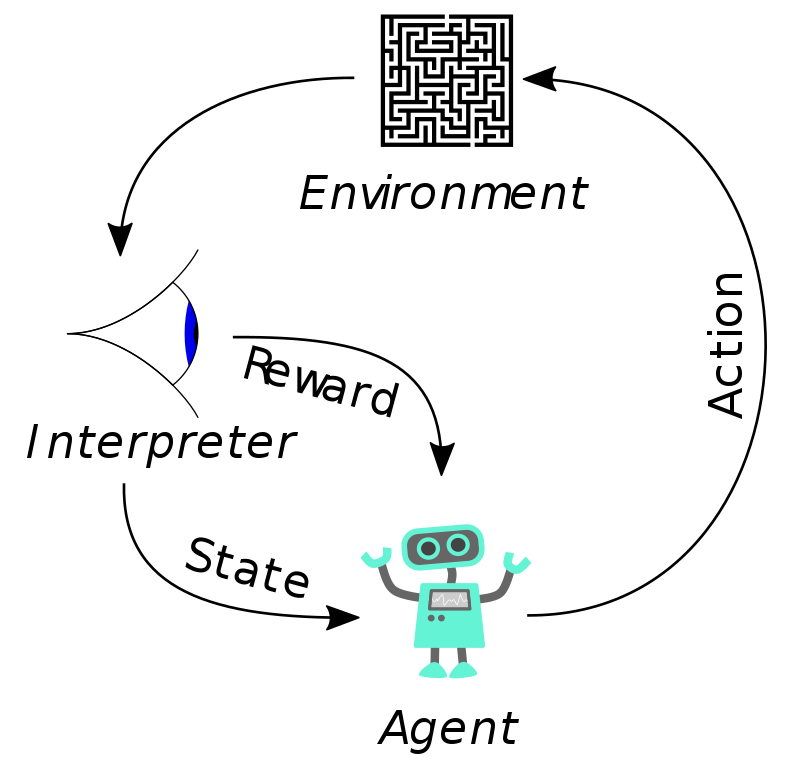
\includegraphics[width=0.5\textwidth]{figs/ch1/Reinforcement_learning_diagram}
\caption{How an agent interacts with the environment.}
\label{fig:deepmind}
\end{figure}

Standard model-based methods for robotic manipulation might involve estimating the physical properties of the environment, and then solving for the controls based on the known laws of physics \cite{OK-Robot-1987} \cite{Predictive2014} \cite{PlanningFramework2012}. This approach has been applied to a range of problems. Despite the extensive work in this area, tasks like pushing an unknown object to a desired position remain a challenging robotic task, largely due to the difficulties in estimating and modeling the physical world \cite{IROS2016}. Learning and optimization-based methods have been applied to various parts of the state-estimation problem, such as object recognition \cite{Visual1995}, pose registration \cite{ObjectRecognition2009}, and dynamics learning \cite{DynamicsDoor2013}.

However, estimating and simulating all of the details of the physical environment is exceedingly difficult, particularly for previously unseen objects, and is arguably unnecessary if the end goal is only to find the desired controls. For example, simple rules for adjusting motion, such as increasing force when an object is not moving fast enough, or the gaze heuristic \cite{FieldersNature2003}, can be used to robustly perform visuomotor control without an overcomplete representation of the physical world and complex simulation calculations. Our work represents an early step toward using learning to avoid the detailed and complex modeling associated with the fully model-based approach.

Several works have used deep neural networks to process images and represent policies for robotic control, initially for driving tasks \cite{AutonomousLand1989} \cite{LongrangeVision2009}, later for robotic soccer \cite{RobotSoccer2009}, and most recently for robotic grasping \cite{Grasp2016} \cite{RooticGrasping2016} and manipulation \cite{Visuomotor2016}. Although these model-free methods can learn highly specialized and proficient behaviors, they recover a task-specific policy rather than a flexible model that can be applied to a wide variety of different tasks. The high dimensionality of image observations presents a substantial challenge to model-based approaches, which have been most successful for low-dimensional non-visual tasks \cite{PolicySearch2011} such as helicopter control \cite{HeliNg2007}, locomotion \cite{Trajectory2012}, and robotic cutting \cite{Deepmpc2015}. Nevertheless, some works have considered modeling high-dimensional images for object interaction. For example, Boots et al. \cite{Predictive2014} learn a predictive model of RGB-D images of a robot arm moving in free space.

% CACC

A lot of related work has been done in recent years in the design of CACC systems. Regarding the vehicle-following controller, Hallouzi et al. [8] did some research as part of the CarTalk 2000 project. These authors worked on the design of a longitudinal CACC controller based on vehicle-to-vehicle communication. They showed that inter-vehicle communication can help reduce instability of a platoon of vehicles. In the same vein, Naranjo and his colleague [14] worked on designing a longitudinal controller based on fuzzy logic. Their approach is similar to what we did with reinforcement learning for our low-level controller. Forbes has presented a longitudinal reinforcement learning controller [5] and compared it to a hand-coded following controller. He showed that the hand-coded controller is more precise than its RL controller but less adaptable in some situations. However, Forbes did not test explicitly communication between vehicles to improve its longitudinal controller to a multi-vehicle environment (which will be the focus of our future work). Our approach will also integrate our low-level controllers with a high-level multiagent decision making algorithm, which was not part of Forbes' work.

Regarding the reinforcement learning in a vehicle coordination problem, Unsal, Kachroo and Bay \cite{CACC1999} have used multiple stochastic learning automata to control the longitudinal and lateral path of a vehicle. However, the authors did not extend their approach to the multi-agent problem. In his work, Pendrith \cite{DistributedRL-Traffic2000} presented a distributed variant of Q-Learning (DQL) applied to lane change advisory system, that is close to the problem described in this paper. His approach uses a local perspective representation state which represents the relative velocities of the vehicles around. Consequently, this representation state is closely related to our 1-partial state representation. Contrary to our algorithms, DQL does not take into account the actions of the vehicles around and updates Q-Values by an average backup value over all agents at each time step. The problem of this algorithm is the lack of learning stability.

On the other hand, our high level controller model is similar to Partially Observable Stochastic Games (POSG). This model formalizes theoretically the observations for each agent. The resolution of this kind of games has been studied by Emery-Montermerlo \cite{GameControl2005}. This resolution is an approximation using Bayesian games. However, this solution is still based on the model of the environment, unlike our approach which does not take into account this information explicitly since we assume that the environment is unknown. Concerning the space search reduction, Sparse Cooperative Q-Learning \cite{Sparse2004} allows agents to coordinate their actions only on predefined set of states. In the other states, agents learn without knowing the existence of the other agents. However, unlike in our approach, the states where the agents have to coordinate themselves are selected statically before the learning process. The joint actions set reduction has been studied by Fulda and Ventura who proposed the Dynamic Joint Action Perception (DJAP) algorithm \cite{JointAction2003}. DJAP allows a multi-agent Q-learning algorithm to select dynamically the useful joint actions for each agent during the learning. However, they concentrated only on joint actions and they tested only their approach on problems with few states.

Introducing communication into decision has been studied by Xuan, Lesser, and Zilberstein \cite{Multi-agentCooperation2001} who proposed a formal extension to Markov Decision Process with communication where each agent observes a part of the environment but all agents observe the entire state. Their approach proposes to alternate communication and action in the decentralized decision process. As the optimal policy computation is intractable, the authors proposed some heuristics to compute approximation solutions. The main differences with our approach is the implicit communication and the model-free learning. More generally, Pynadath and Tambe \cite{Communicative2002} have proposed an extension to distributed POMDP with communication called COM-MTDP, which take into account the cost of communication during the decision process. They presented complexity results for some classes of team problems. As Xuan, Lesser, and Zilberstein \cite{Multi-agentCooperation2001}, this approach is mainly theoretical and does not present model-free learning. The locality of interactions in a MDP has been theoretically developed by Dolgov and Durfee \cite{Makov2004}. They presented a graphical approach to represent the compact representation of a MDP. However, their approach has been developed to solve a MDP and not to solve directly a multi-agent reinforcement learning problem where the transition function is unknown.


\section{Thesis Outline}

The goal of this thesis is to provide operational specifications for the development of a level 4 capable AVRP. This section will present the chapters and subsections of this thesis and provide a brief summary of those sections.

Chapter 2 details the system specifications required to develop an AVRP, based off feedback from faculty and researchers at Virginia Tech.
\begin{itemize}
\item \textbf {Section 2.1 Interdisciplinary Design Needs:} Looks at the feedback given by faculty and researchers at Virginia Tech and what kinds of research they would like to utilize an AVRP for. Breaks down the research desires into the basic needs for an AVRP. Some of the feedback is broken down with more background information.
\end{itemize}

Chapter 3 dives into the hardware and sensing side of an AVRP and lays out a discussion of the technology needed, such as DBW, navigation, sensing, communication, computing, power bus, and external mounting racks. It then reviews additional design considerations that need to be taken into consideration when designing an AVRP. Chapter 3 is laid out as follows:
\begin{itemize}
\item \textbf {Section 3.1 Drive By Wire:} Discusses the DBW system and significant design parameters to be considered. Lays out the specifications of the by wire system on a base platform at Virginia Tech. Presents a high level overview of DBW system.
\item \textbf {Section 3.2 Navigation:} Discusses different combinations for navigation, such as GPS/ INS and GPS/IMU, and some of the characteristics associated with each, as well as navigation via dead reckoning. Correction techniques such as DGPS and DGPS with RTK are reviewed. Hardware mounting is briefly mentioned.
\item \textbf {Section 3.3.1 LIDAR:} Discusses how LIDAR works. 2D and 3D LIDAR is discussed. Discusses certain characteristics such as range, accuracy, field of view, number of re- turns, intensity, advantages and disadvantages. Reviews possible mounting locations.
\item \textbf {Section 3.3.2 Radar:} Discusses how radar works and its usefulness on an AVRP. Talks about the different operation frequencies used in autonomy and how they affect performance, as well as other advantages and disadvantages. Possible mounting locations are discussed.
\item \textbf {Section 3.3.3 Ultrasonic:} Discusses the use of ultrasonic sensors and their advantages and disadvantages. Reviews their range and mounting locations.
\item \textbf {Section 3.3.4 Cameras:} Discusses different camera types and capability they bring to an AVRP. Goes over camera specifications for consideration. Reviews potential mounting locations.
\item \textbf {Section 3.3.5 Wheel Speed and Steering Angle Sensors: }Discusses wheel encoders and steering angle sensors and how they complement other sensing and systems.
\item \textbf {Section 3.4.1 Communication:} Presents different communication buses for intra-vehicle communication. Provides an overview, specs, and explanation of an AVRP communication bus structure. Reviews the need for an emergency stop system.
\item \textbf {Section 3.4.2 Computers:} Addresses computing for the end users by presenting bench- marks and guide posts for consideration when determining computational needs for the end user of an AVRP.
\item \textbf {Section 3.5 Base Sensor Suite Design:} Specs out the base sensor suite for an AVRP and the capabilities it allows for the AVRP without user added sensors.
\item \textbf {Section 3.6 Power Bus:} Discusses AVRP power bus layout to provide power to all internally and externally mounted hardware and sensors. Provides an estimate of power need for base sensor suite and an example sensor suite.
\item \textbf {Section 3.7.1 Front Universal Mounting Racks:} Reviews details and modifications made for adding front universal mounting rack to AVRP.
\item \textbf {Section 3.7.2 Rear Universal Mounting Racks:} Reviews details and modifications made for adding rear universal mounting rack to AVRP.
\item \textbf {Section 3.7.3 Roof Universal Mounting Racks:} Reviews details and modifications made for adding roof top universal mounting rack to AVRP.
\item \textbf {Section 3.7.4 Mounting Rack Vibration:} Discusses vibration concerns and performs example natural frequency calculations for the front and rear universal mounting racks.
\item \textbf {Section 3.7.5 Interchanging Hardware:} Discusses design considerations for hardware and sensors to be added to the mounting racks, such as roof top penetrations, routing wires, adapter brackets, etc.
\item \textbf {Section 3.8 Additional Design Considerations:} Discusses other AVRP design considerations, such as funding, team structure, base vehicle variability, hardware selection properties, etc.
\end{itemize}

Chapter 4 reviews the base vehicle research capabilities and contains a testing plan ideas for an AVRP. Chapter 4 is a follows:

\begin{itemize}
\item \textbf {Section 4.1 Base Vehicle Research Capabilities:} Reiterates on the base platform capabilities without any user added sensors.
\item \textbf {Section 4.2 Testing Plan Overview:} Discusses testing plan options for an AVRP and how it can be validated for use for its researchers.
\end{itemize}

Chapter 5 contains the conclusion and areas for future work. Chapter 5 sections are as follows:

\begin{itemize}
\item \textbf {Section 5.1 Conclusion:} Reviews the design of an AVRP, hardware, sensors, and modifications to make it adaptable to a researcher?s needs.
\item \textbf {Section 5.2 Future Work:} Looks at areas relevant to an AVRP in which further research can be conducted.
\end{itemize}

%%%%%%%%%%%%%%%%%%%%%%%%%%%%%%%%%%%%%%%%%%%%%%%%%%%%%%%%%%%%%%%%%%%%%%%%%%%%%%%%%%%%%%%%%%%%%%%%%%%%



%\bibliographystyle{plainnat}
%\markright{\textit{Bibliography}}
%\renewcommand{\chaptername}{}
%x\bibliography{KL-Thesis}

\vfill


%background
\chapter{Simulated Environment} 

% 

In order for autonomous vehicles to operate safely in the real world, they must be able to adapt to a multitude of changing conditions. Before fully self-driving vehicles hit the road, they undergo a lengthy period of testing where the vehicle's sensors and artificial intelligence are tested in a variety of simulated real-world environments. Simulation has become the backbone of the autonomous driving industry, providing a means to collect extensive amounts of data for model training as well as providing a safe testbed to crash-test these models. In this chapter, we would like to create a simulator for training autonomous diving algorithms.

A simplified highway environment would be created to train deep learning models for the autonomous vehicle to gain better decision making ability of speed control and  lane changing.

The simulated environment is constructed based on ROS and Gazebo and the Reinforcement Learning Algorithms are implemented by OpenAI-Gym. An open source car model kit, Drive-by-Wire (DBW) Kit, is adopted to play the role of the autonomous vehicle. An overall architecture of the simulation environment is shown as Fig. \ref{fig:sim-env}.

\begin{figure}[h]
\centering
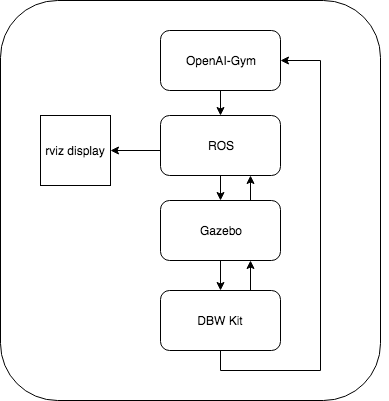
\includegraphics[width=0.7\textwidth]{figs/ch2/simulation-architecture}
\caption{Architecture of the simulation environment.}
\label{fig:sim-env}.
\end{figure}

% why openai-gym

OpenAI was founded in late 2015 as a non-profit with a mission to "build safe artificial general intelligence (AGI) and ensure AGI's benefits are as widely and evenly distributed as possible." In addition to exploring many issues regarding AGI, one major contribution that OpenAI made to the machine learning world was developing both the Gym and Universe software platforms. OpenAI-Gym is a collection of environments / problems designed for testing and developing reinforcement learning algorithms --- it saves the user from having to create complicated environments. Gym is written in Python, and there are multiple environments such as robot simulations or Atari games. There is also an online leaderboard for people to compare results and code.

% why ros

% why gazebo

The usual basic requirements to robot simulators are an accurate physics simulation (such as object velocity, inertia, friction, position and orientation, etc.), high quality rendering (for shape, dimensions, colors, and texture of objects), integration with the Robot Operating System (ROS) framework and multi-platform performability. It provides great opportunities for modeling robots and their sensors together with developing robot control algorithms, realizing mobile robot simulation, visualization, locomotion and navigation in a realistic 3D environment. As mentioned in the paper \cite{jmeSim2012}, the high graphical fidelity in a robot simulation is important because the sensory input to the robot perceptual algorithms comes from virtual sensors, which are also provided by the simulation. For example, virtual cameras use the simulator rendering engine to obtain their images. If images from a simulated camera have incorrect similarity to real camera ones, then it is not possible to use them for object recognition and localization.

To avoid such a sort of problems, we use the robust and high graphical quality robot simulator --- Gazebo, which is an open source robotic simulation package that closely integrated with ROS. Gazebo uses the open source OGRE rendering engine, which produces good graphics fidelity, although it also employs the Open Dynamics Engine (ODE), which is estimated as slow physics engine \cite{jmeSim2012}.

%%%%%%%%%%%%%%%%%%%%%%%%%%%%%%%%%%
\section{ROS}

Writing software for robots is difficult, particularly as the scale and scope of robotics continues to grow. Different types of robots can have wildly varying hardware, making code reuse nontrivial. A wide variety of frameworks were created to liberate researchers and developers from those way beyond their interests. Among them, Robot Operating System (ROS) framework \cite{ROS2009}  gained more popularity because of its generality and expansibility. ROS was designed to meet a specific set of challenges encountered when developing large-scale service robots as part of the STAIR project \cite{STAIR2007} at Stanford University and the Personal Robots Program \cite{PR2008} at Willow Garage, but the resulting architecture is far more general than the service-robot and mobile-manipulation domains.

The philosophical goals of ROS can be summarized as:

\begin{itemize}
\item Peer-to-peer 
\item Tools-based 
\item Multi-lingual 
\item Thin
\item Free and Open-Source
\end{itemize}

\subsection{Implementation}

The fundamental concepts of the ROS implementation are nodes, messages, topics, and services.

Nodes are processes that perform computation. ROS is designed to be modular at a fine-grained scale: a system is typically comprised of many nodes. In this context, the term "node" is interchangable with "software module". Our use of the term "node" arises from visualizations of ROS-based systems at runtime: when many nodes are running, it is convenient to render the peer-to-peer communications as a graph, with processes as graph nodes and the peer-to-peer links as arcs.

Nodes communicate with each other by passing messages. A message is a strictly typed data structure. Standard primitive types (integer, floating point, boolean, etc.) are supported, as are arrays of primitive types and constants. Messages can be composed of other messages, and arrays of other messages, nested arbitrarily deep.

A node sends a message by publishing it to a given topic, which is simply a string such as "odometry" or "map". A node that is interested in a certain kind of data will subscribe to the appropriate topic. There may be multiple concurrent publishers and subscribers for a single topic, and a single node may publish and/or subscribe to multiple topics. In general, publishers and subscribers are not aware of each others' existence.

\begin{figure}[h]
\centering
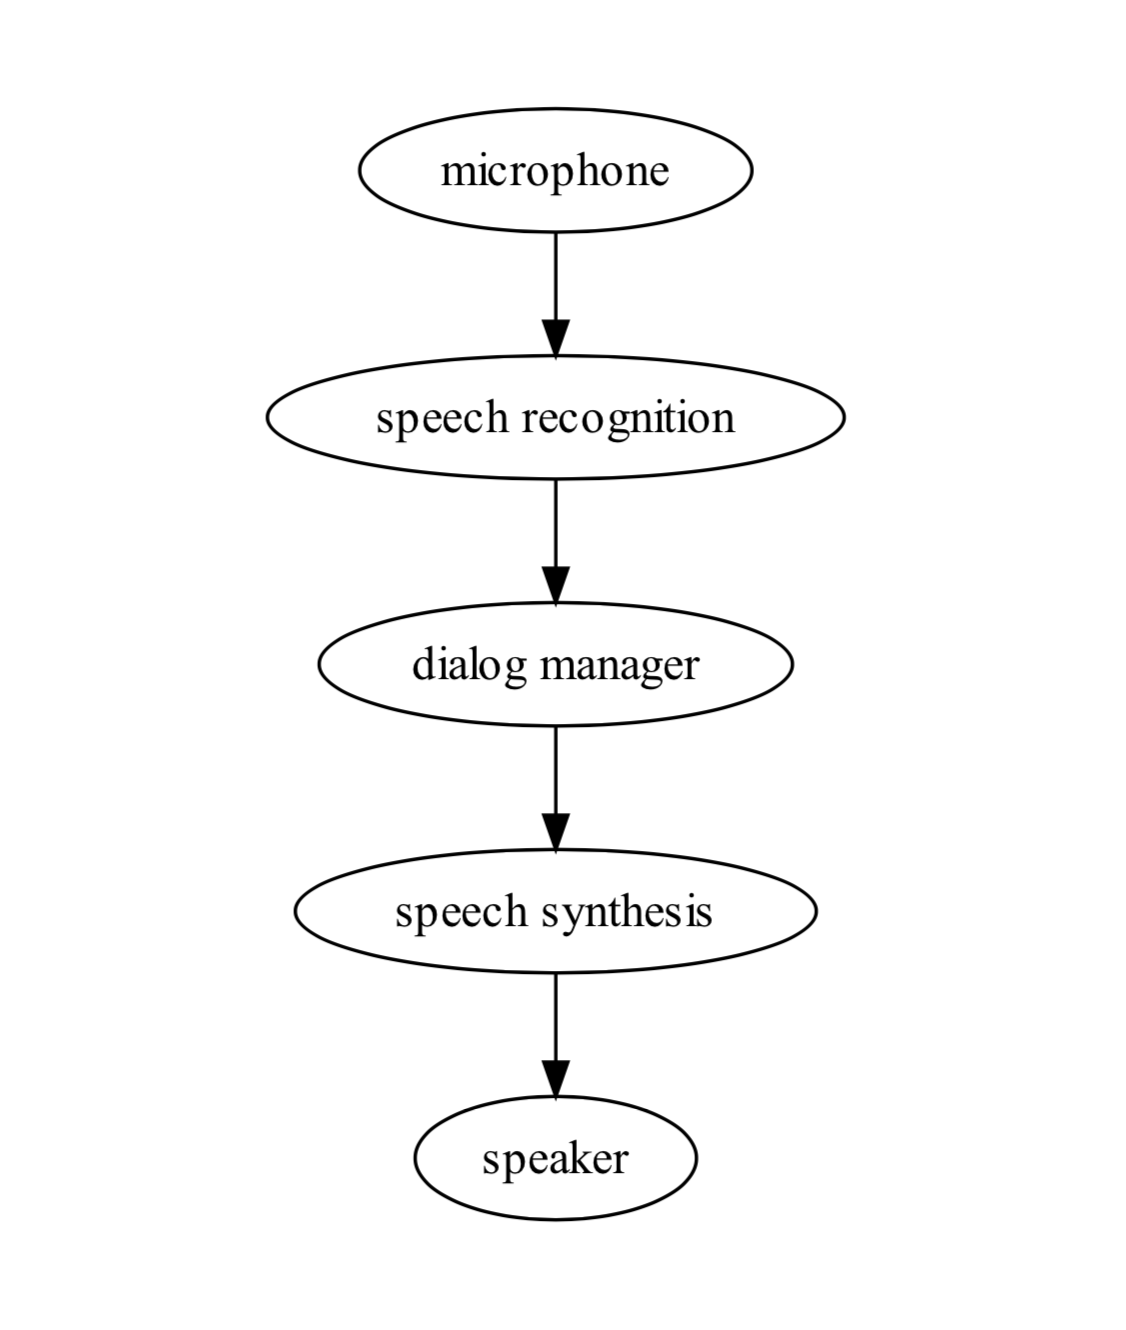
\includegraphics[width=0.6\textwidth]{figs/ch2/ros-pipeline}
\caption{Communication pipeline.}
\end{figure}

\subsection{Collaborative Development}

Due to the vast scope of robotics and artificial intelligence, collaboration between modules is necessary in order to build large systems. To support collaborative development, the ROS software system is organized into packages. Here the definition of "package" is deliberately open-ended: a ROS package is simply a directory which contains an XML file describing the package and stating any dependencies.

A collection of ROS packages is a directory tree with ROS packages at the leaves: a ROS package repository may thus contain an arbitrarily complex scheme of subdirectories. For example, one ROS repository has root directories including "nav", "vision" and "motion planning" each of which contains many packages as subdirectories.

The open-ended nature of ROS packages allows for great variation in their structure and purpose: some ROS packages wrap existing software, such as Player or OpenCV, automating their builds and exporting their functionality. Some packages build nodes for use in ROS graphs, other packages provide libraries and standalone executables, and still others provide scripts to automate demonstrations and tests. The packaging system is meant to partition the building of ROS-based software into small, manageable chunks, each of which can be maintained and developed on its own schedule by its own team of developers.

\subsection{Visualization and Monitoring}

While designing and debugging robotics software, it often becomes necessary to observe some state while the system is running. Although \textit{printf} is a familiar technique for debugging programs on a single machine, this technique can be difficult to extend to large-scale distributed systems, and can become unwieldy for general-purpose monitoring.

Instead, ROS can exploit the dynamic nature of the connectivity graph to "tap into" any message stream on the system. Furthermore, the decoupling between publishers and subscribers allows for the creation of general-purpose visualizers. Simple programs can be written which subscribe to a particular topic name and plot a particular type of data, such as laser scans or images. However, a more powerful concept is a visualization program which uses a plugin architecture: this is done in the \textit{rviz} program, which is distributed with ROS. Visualization panels can be dynamically instantiated to view a large variety of datatypes, such as images, point clouds, geometric primitives (such as object recognition results), render robot poses and trajectories, etc. Plugins can be easily written to display more types of data.

A native ROS port is provided for Python, a dynamically-typed language supporting introspection. Using Python, a powerful utility called \textit{rostopic} was written to filter messages using expressions supplied on the command line, resulting in an instantly customizable "message tap" which can convert any portion of any data stream into a text stream. These text streams can be piped to other UNIX command-line tools such as \textit{grep}, \textit{sed}, and \textit{awk}, to create complex monitoring tools without writing any code.

Similarly, a tool called \textit{rxplot} provides the functionality of a virtual oscilloscope, plotting any variable in real-time as a time series, again through the use of Python introspection and expression evaluation.

\subsection{Transformations}

Robotic systems often need to track spatial relationships for a variety of reasons: between a mobile robot and some fixed frame of reference for localization, between the various sensor frames and manipulator frames, or to place frames on target objects for control purposes.

To simplify and unify the treatment of spatial frames, a transformation system has been written for ROS, called \textit{tf}. The \textit{tf} system constructs a dynamic transformation tree which relates all frames of reference in the system. As information streams in from the various subsystems of the robot (joint encoders, localization algorithms, etc.), the \textit{tf} system can produce streams of transformations between nodes on the tree by constructing a path between the desired nodes and performing the necessary calculations.

For example, the \textit{tf} system can be used to easily generate point clouds in a stationary "map" frame from laser scans received by a tilting laser scanner on a moving robot. As another example, consider a two-armed robot: the \textit{tf} system can stream the transformation from a wrist camera on one robotic arm to the moving tool tip of the second arm of the robot. These types of computations can be tedious, error- prone, and difficult to debug when coded by hand, but the \textit{tf} implementation, combined with the dynamic messaging infrastructure of ROS, allows for an automated, systematic approach.

%%%%%%%%%%%%%%%%%%%%%%%%%%%%%%%%%%
\section{Gazebo}

Gazebo is a 3D dynamic simulator with the ability to accurately and efficiently simulate populations of robots in complex indoor and outdoor environments, which makes it possible to rapidly test algorithms, design robots, perform regression testing, and train AI system using realistic scenarios. While similar to game engines, Gazebo offers physics simulation at a much higher degree of fidelity, a suite of sensors, and interfaces for both users and programs. Fig. \ref{fig:pr2} gives a typical display of Gazebo and in the window is a PR2 robot \cite{PR2008} with its LIDAR sensor range displayed in blue.

\begin{figure}[h]
\centering
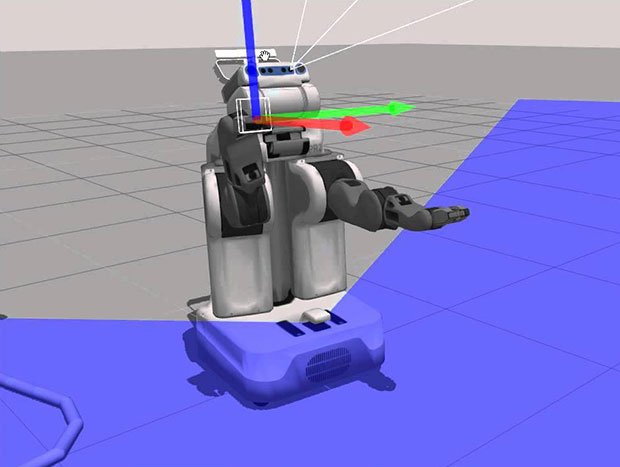
\includegraphics[width=0.8\textwidth]{figs/ch2/osrf.jpeg}
\caption{Gazebo for robot simulation.}
\label{fig:pr2}
\end{figure}

Typical uses of Gazebo include:

\begin{itemize}
\item testing robotics algorithms,
\item designing robots,
\item performing regression testing with realistic scenarios
\end{itemize}

A few key features of Gazebo include:

\begin{itemize}
\item multiple physics engines,
\item a rich library of robot models and environments,
\item a wide variety of sensors,
\item convenient programmatic and graphical interfaces
\end{itemize}

Gazebo is far from being the only choice for a 3D dynamics simulator. It is however one of the few that attempts to create realistic worlds for the robots rather than just human users. As more advanced sensors are developed and incorporated into Gazebo the line between simulation and reality will continue to blur, but accuracy in terms of robot sensors and actuators will remain an overriding goal.

\subsection{Architecture}

Gazebo's architecture has progressed through a couple iterations during which we learned how to best create a simple tool for both developers and end users. We realized from the start that a major feature of Gazebo should be the ability to easily create new robots, actuators, sensors, and arbitrary objects. As a result, Gazebo maintains a simple API for addition of these objects, which we term models, and the necessary hooks for interaction with client programs. A layer below this API resides the third party libraries that handle both the physics simulation and visualization. The particular libraries used were chosen based on their open source status, active user base, and maturity.

\begin{figure}[h]
\centering
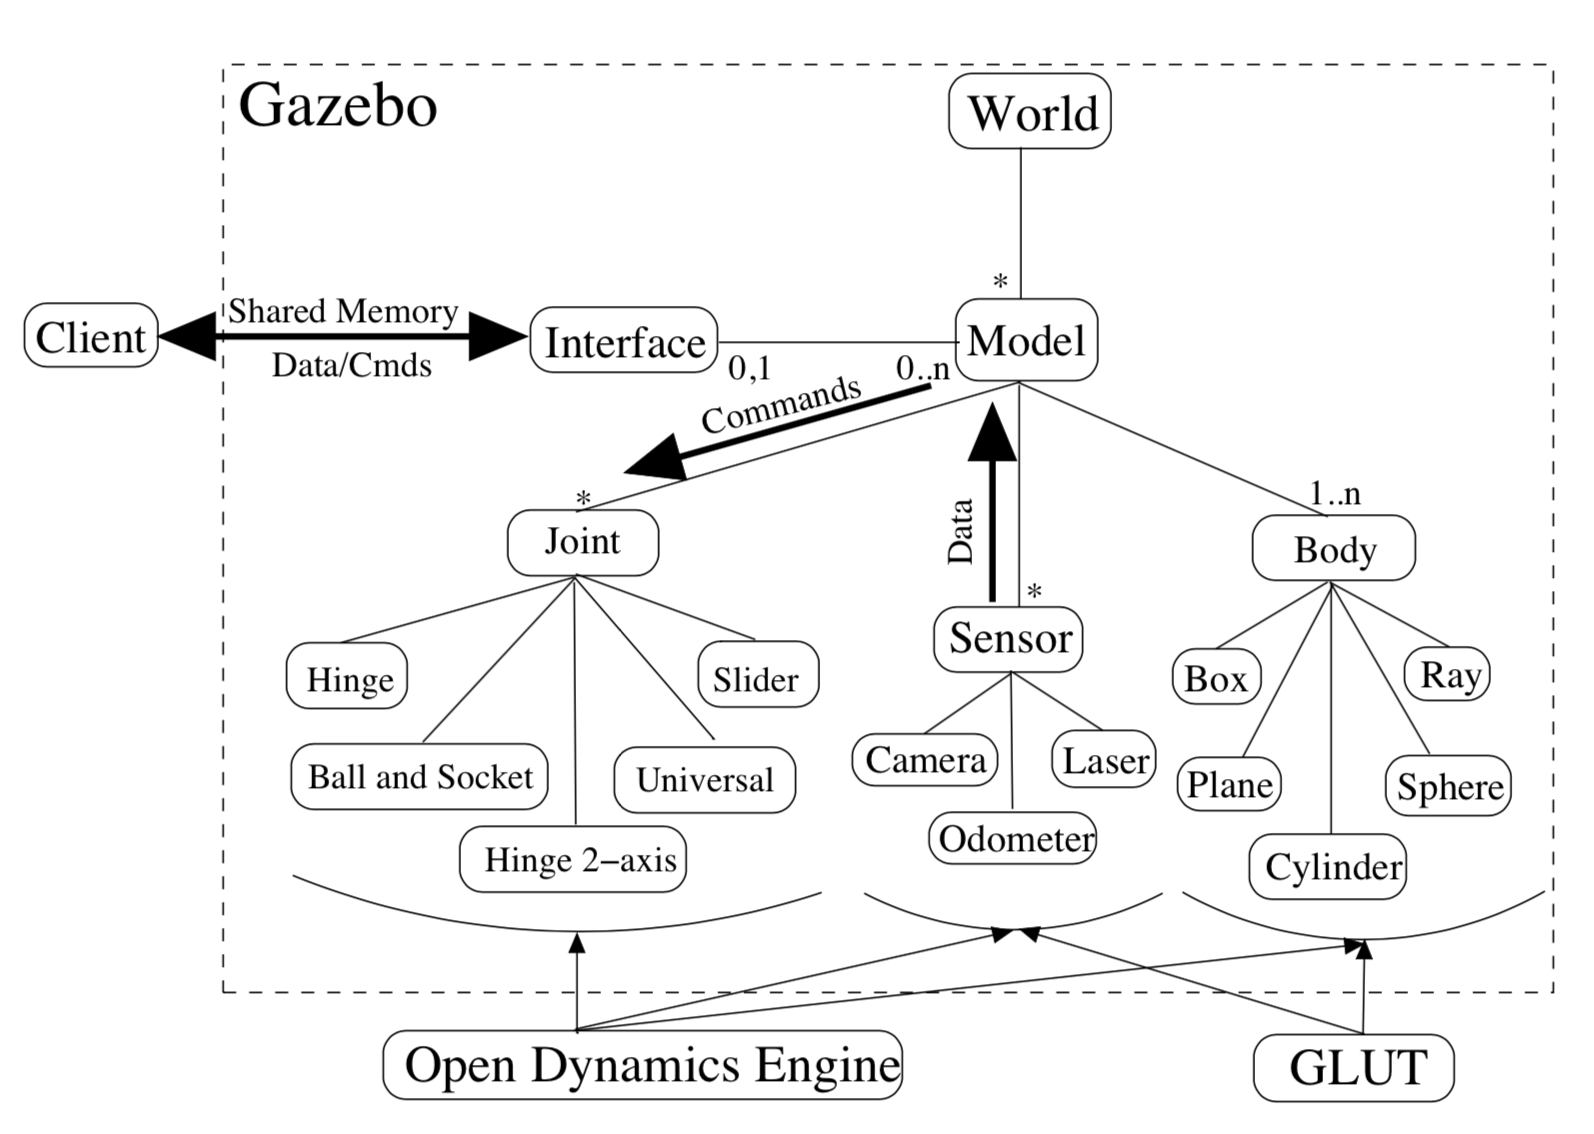
\includegraphics[width=0.8\textwidth]{figs/ch2/gazebo-structure}
\caption{Gazebo's architecture.}
\label{fig:gazebo-structure}
\end{figure}

This architecture is graphically depicted in Fig. \ref{fig:gazebo-structure}. The World represents the set of all models and environmental factors such as gravity and lighting. Each model is composed of at least one body and any number of joints and sensors. The third party libraries interface with Gazebo at the lowest level. This prevents models from becoming dependent on specific tools that may change in the future. Finally, client commands are received and data returned through a shared memory interface. A model can have many interfaces for functions involving, for example, control of joints and transmission of camera images.

\subsection{Physics Engine}

The Open Dynamics Engine, created by Russel Smith is a widely used physics engine in the open source community. It is designed to simulate the dynamics and kinematics associated with articulated rigid bodies. This engine includes many features such as numerous joints, collision detection, mass and rotational functions, and many geometries including arbitrary triangle meshes. Gazebo utilizes these features by providing a layer of abstraction situated between ODE and Gazebo models. This layer allows easy creation of both normal and abstract objects such as laser rays and ground planes while maintaining all the functionality provided by ODE. %With this internal abstraction, it is possible to replace the underlying physics engine, should a better alternative become available.

\subsection{Visualization}

A well designed simulator usually provides some form of user interface, and Gazebo requires one that is both sophisticated and fast. The heart of Gazebo lies in its ability to simulate dynamics, and this requires significant work on behalf of the user's computer. A slow and cumbersome user interface would only detract from the simulator's primary purpose. To account for this, OpenGL and GLUT (OpenGL Utility Toolkit) were chosen as the default visualization tools.

OpenGL is a standard library for the creation of 2D and 3D interactive applications. It is platform independent, highly scalable, stable, and continually evolving. More importantly, many features in OpenGL have been implemented in graphic card hardware thereby freeing the CPU for other work such as the computationally expensive dynamics engine.

GLUT is a simple window system independent toolkit for OpenGL applications. Scenes rendered using OpenGL are displayed in windows created by GLUT. This toolkit also provides mechanisms for user interaction with Gazebo via standard input devices such as keyboards and mice. GLUT was chosen as the default windowing toolkit be- cause it is lightweight, easy to use, and platform independent.

\subsection{Customized Environment}

A complete environment is essentially a collection of models and sensors. The ground and buildings represent stationary models while robots and other objects are dynamic. Sensors remain separate from the dynamic simulation since they only collect data, or emit data if it is an active sensor.

\textbf{Models:} A model is any object that maintains a physical representation, which can be created by hand. The process starts with choosing the appropriate bodies and joints necessary to build an accurate model in both appearance and functionality. This encompasses anything from simple geometry to complex robots. Models are composed of at least one rigid body, zero or more joints and sensors, and interfaces to facilitate the flow of data.

Bodies represent the basic building blocks of a model. Their physical representation take the form of geometric shapes chosen from boxes, spheres, cylinders, planes, and lines. Each body has an assigned mass, friction, bounce factor, and rendering properties such as color, texture, transparency, etc.

Joints provide the mechanism to connect bodies together to form kinematic and dynamic relationships. A variety of joints are available including hinge joints for rotation along one or two axis, slider joints for translation along a single axis, ball and socket joints, and universal joints for rotation about two perpendicular joints. Besides connecting two bodies together, these joints can act like motors. When a force is applied to a joint, the friction between the connected body and other bodies cause motion. However, special care needs to be taken when connecting many joints in a single model as both the model and simulation can easily loose stability if incorrect parameters are chosen.

Interfaces provide the means by which client programs can access and control models. Commands sent over an interface can instruct a model to move joints, change the configuration of associated sensors, or request sensor data. The interfaces do not place restrictions on a model, thereby allowing the model to interpret the commands in anyway it sees fit.

\textbf{Sensors:} A robot can't perform useful tasks without sensors. A sensor in Gazebo is an abstract device lacking a physical representation. It only gains embodiment when incorporated into a model. This feature allows for the reuse of sensors in numerous models thereby reducing code and confusion.

There currently are three sensor implementations including an odometer, ray proximity, and a camera. Odometry is easily accessible through integration of the distance traveled. The ray proximity sensor returns the contact point of the closest object along the ray's path.

\textbf{External Interfaces:} From the users point of view, the models simulated in Gazebo are the same as their real counterparts, and are treated as a normal device capable of sending and receiving data. A second key advantage to this approach is that one can use abstract drivers inside a simulation. 

The low-level library provides a mechanism for any third-party robot device server interface with Gazebo. Going even further, a connection to the the library is not even necessary since Gazebo can be run independently for rapid model and sensor development. Currently the Gazebo library offers hooks to set wheel velocities, read data from a laser range finder, retrieve images from a camera, and insert simple objects into the environment at runtime. This data is communicated through shared memory for speed and efficiency.

\textbf{Environments:} Many environments in which robots operate are either well studied or carefully constructed. Deploying robots in a never before encountered world may cause unforeseen, and possibly negative, side effects. Lighting conditions, reflective surfaces, and odd objects can all play an effect on how a robot operates. A strategy of online testing can be extremely slow and tedious. Time can be spent much more productively by testing and modifying the robot controllers offline in preparation for the real experiments. The fine grained control of Gazebo, the ability to extrude 2D images into 3D structures, and terrain generation allow for the unique ability to hand create rough outlines of a new environment. 

As a result, the development time of the algorithms employed was greatly reduced. Gazebo made it possible to continue experimentation in the environment even after the physical robots were deployed. Elevation information collected by real sensors can be imported along with relevant structures to further blur the line between simulation and the real world. All of this culminates in the ability of Gazebo to reduce development and test time, and even allow experiments to virtually take place in almost any part of the world.

\subsection{Test Bed for Algorithm Design}

The design and implementation of new algorithms can be a difficult task that become particularly acute with the lack of convenient test environments. In situations such as this, Gazebo's sensory realism can play a time saving role. Traditionally, development of new algorithms either required custom simulators or direct testing on the hardware; Gazebo's realistic environments and simple interface can drastically reduce the turn around time from a conceptual stage to functional system.

%%%%%%%%%%%%%%%%%%%%%%%%%%%%%%%%%%
\section{OpenAI-Gym}

Reinforcement learning assumes that there is an agent that is situated in an environment. Each step, the agent takes an action, and it receives an observation and reward from the environment. An RL algorithm seeks to maximize some measure of the agent's total reward, as the agent interacts with the environment. In the RL literature, the environment is formalized as a partially observable Markov decision process (POMDP) \cite{Sutton1998RL}.

OpenAI Gym focuses on the episodic setting of reinforcement learning, where the agent's experience is broken down into a series of episodes. In each episode, the agent's initial state is randomly sampled from a distribution, and the interaction proceeds until the environment reaches a terminal state. The goal in episodic reinforcement learning is to maximize the expectation of total reward per episode, and to achieve a high level of performance in as few episodes as possible.

OpenAI Gym aims to combine the best elements of these previous benchmark collections, in a software package that is maximally convenient and accessible. It includes a diverse collection of Environments (POMDPs) with a common interface, and this collection will grow over time. The environments are versioned in a way that will ensure that results remain meaningful and reproducible as the software is updated.

\subsection{Design For Environment}

The design of OpenAI Gym is based on the experience developing and comparing reinforcement learning algorithms, and the experience using previous benchmark collections. Below, we will summarize some of our design decisions.

Two core concepts in Reinforcement Learning are the agent and the environment. OpenAi Gym's design focuses on providing an abstraction for the environment, but not for the agent. This choice was to maximize convenience for users and allow them to implement different styles of agent interface. First, one could imagine an ``online learning'' style, where the agent takes (observation, reward, done) as an input at each time-step and performs learning updates incrementally. In an alternative ``batch update'' style, a agent is called with observation as input, and the reward information is collected separately by the RL algorithm, and later it is used to compute an update. By only specifying the agent interface, it is allowed to write customized agents with either of these styles.

\subsection{Interfacing with ROS and Gazebo}

In the context of robotics, reinforcement learning offers a framework for the design of sophisticated and hard-to-engineer behaviors \cite{RLsurvey2013}. The challenge is to build a simple environment where this machine learning techniques can be validated, and later applied in a real scenario.

OpenAI Gym leaves interfaces to write customized agents, which makes it possible to integrate the Gym API with robotic hardware, validating reinforcement learning algorithms in real environments. The robotic operation is achieved combining Gazebo simulator with ROS.

\begin{figure}[h]
\centering
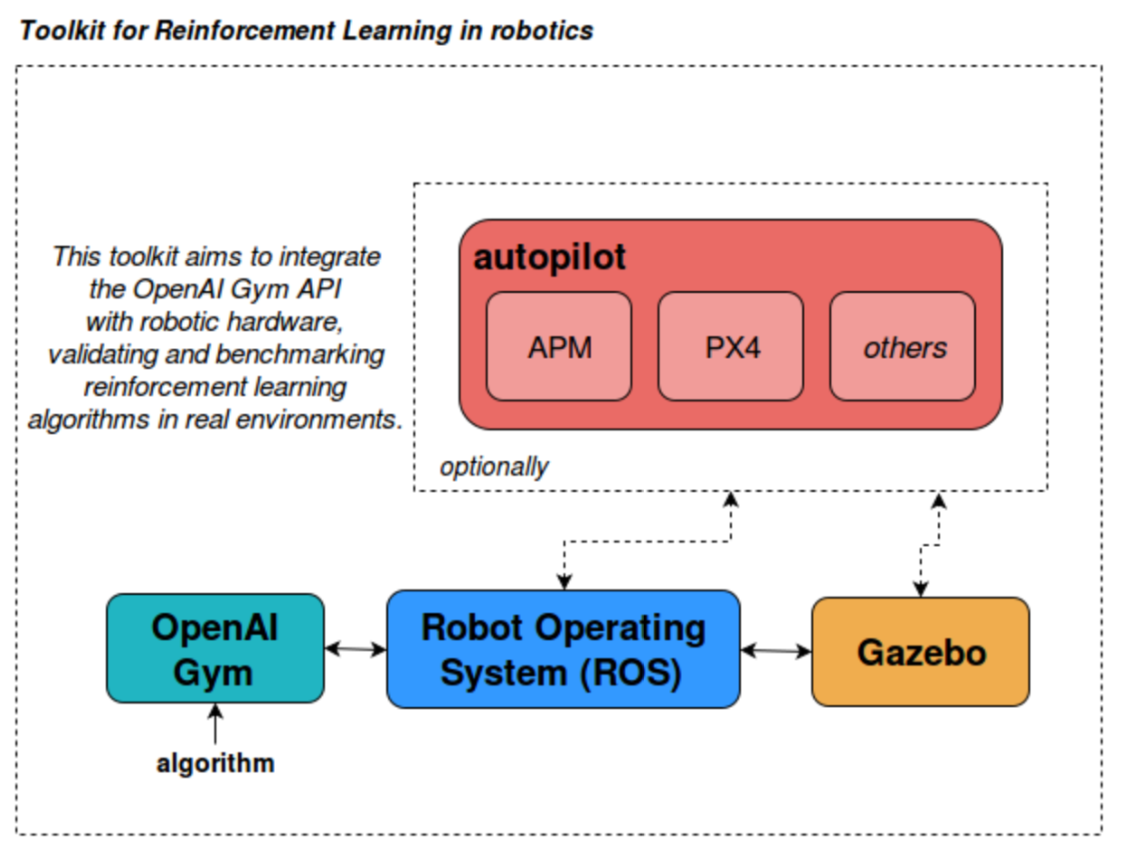
\includegraphics[width=0.8\textwidth]{figs/ch2/toolkit-of-openaigym}
\caption{Simplified software architecture used in OpenAI Gym for robotics.}
\label{fig:openai-archi}
\end{figure}

The architecture consists of three main software blocks: OpenAI Gym, ROS and Gazebo as shown in Fig. \ref{fig:openai-archi}. Environments developed in OpenAI Gym interact with ROS, which is the connection between the Gym itself and Gazebo simulator. Gazebo provides a robust physics engine, high-quality graphics, and convenient programmatic and graphical interfaces.

The physics engine needs a robot definition in order to simulate it, which is provided by ROS or a Gazebo plugin that interacts with an autopilot in some cases (depends on the robot software architecture).

\subsection{Example Use: Train a Cart-pole agent}

\begin{figure}[h]
\centering
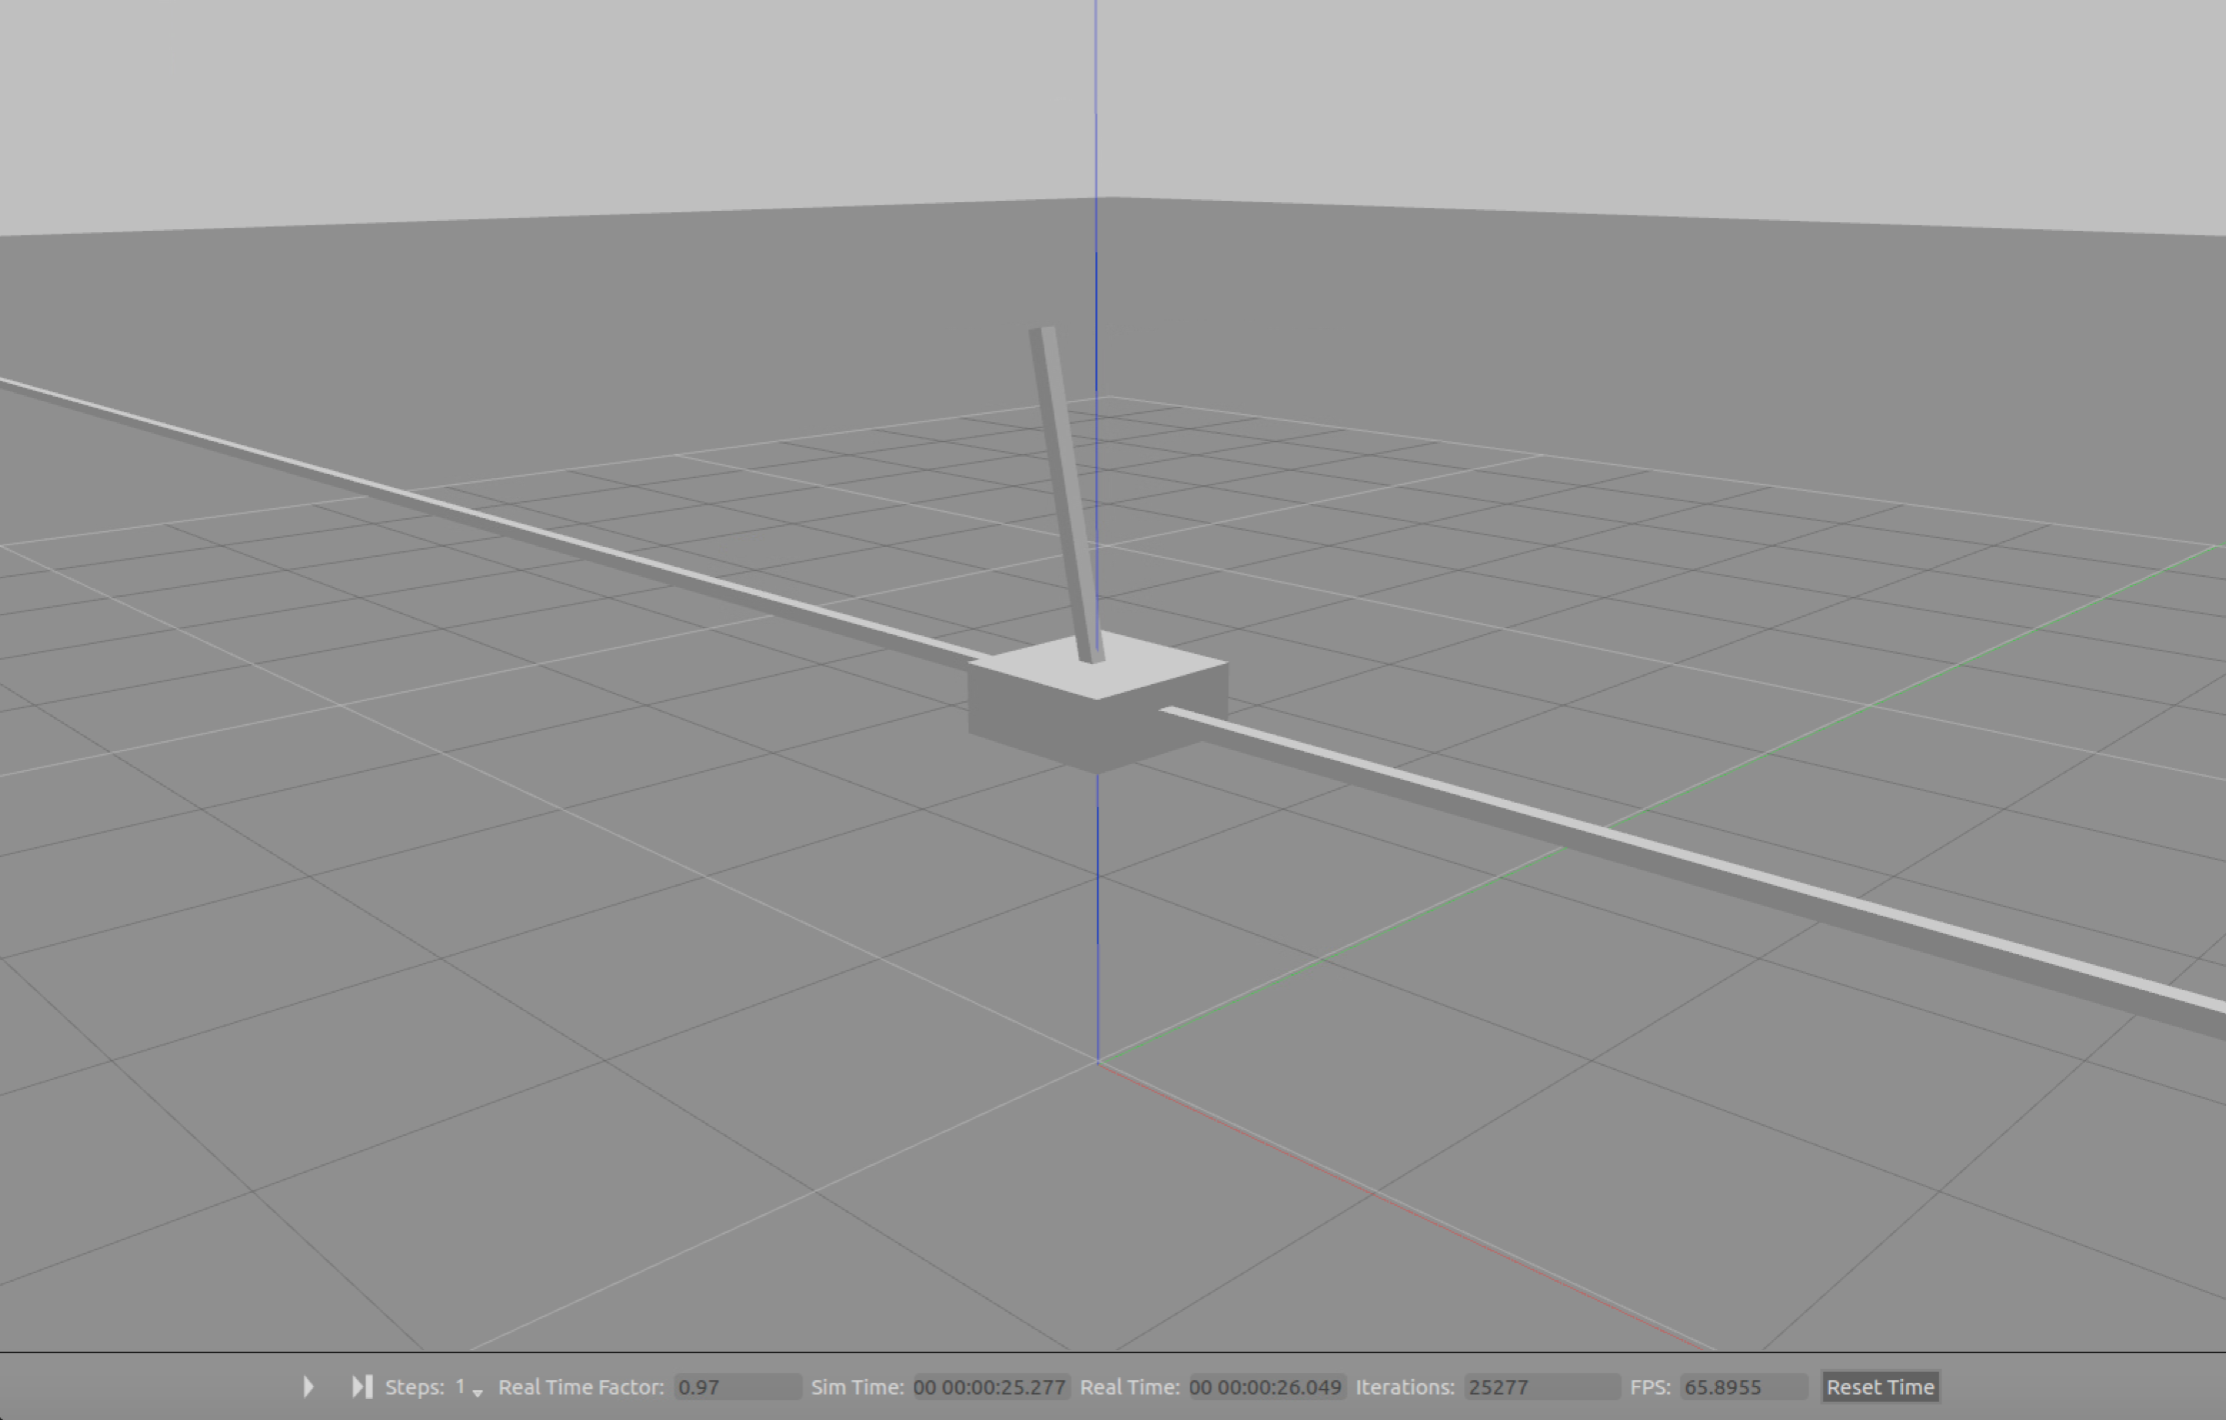
\includegraphics[width=0.8\textwidth]{figs/ch2/cartpole-in-gazebo}
\caption{A Cart-pole model created in Gazebo.}
\label{fig:cartpole-in-gazebo}
\end{figure}

\begin{figure}[h]
\centering
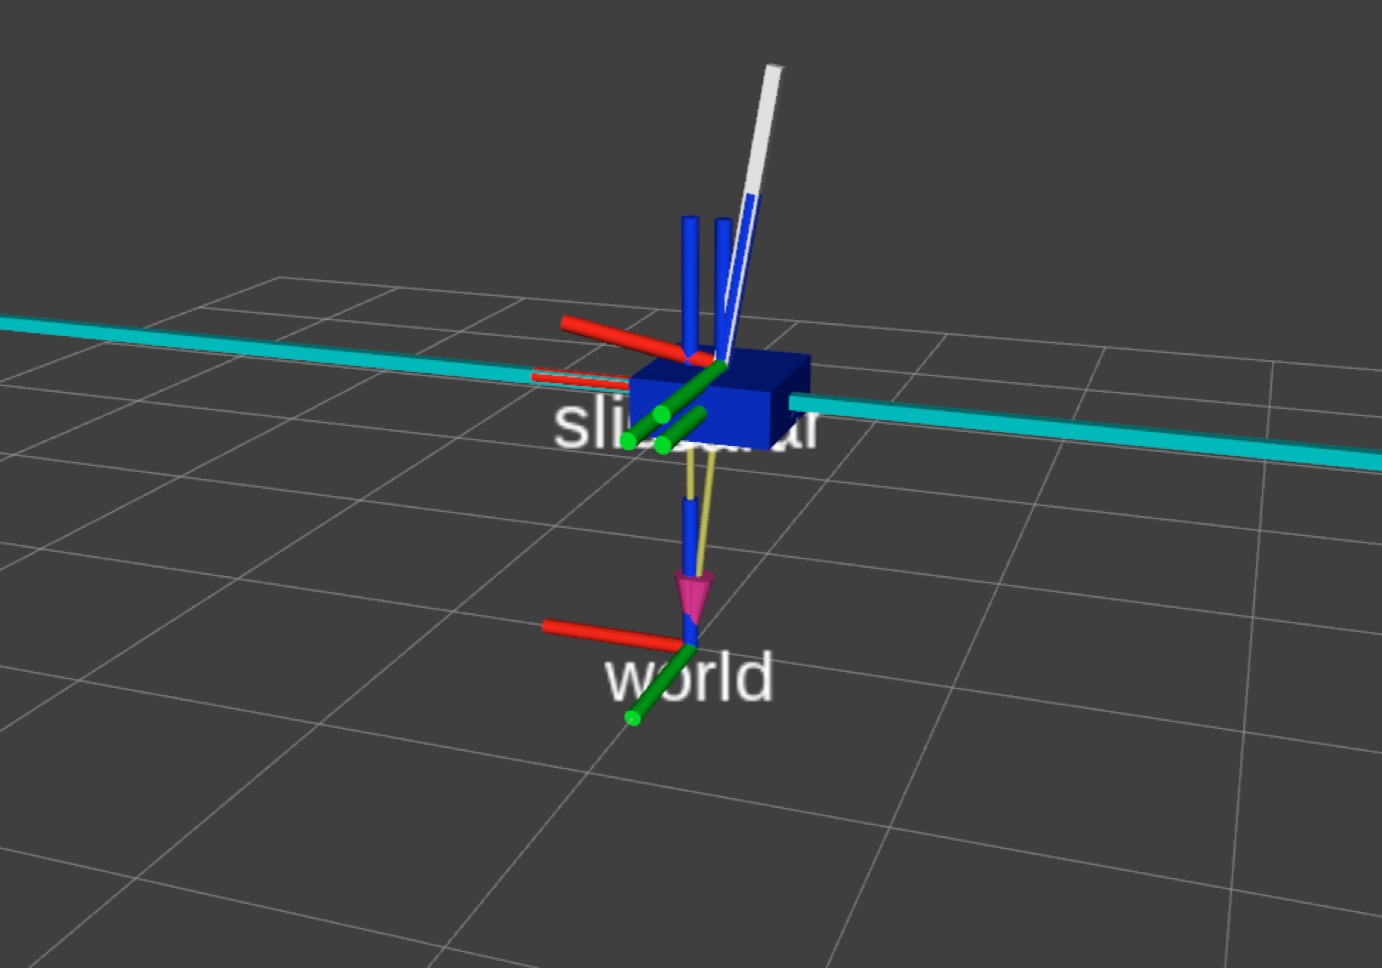
\includegraphics[width=0.8\textwidth]{figs/ch2/cartpole-in-rviz}
\caption{A Cart-pole model displayed in ROS-Rviz.}
\label{fig:cartpole-in-rviz}
\end{figure}

Before we dive into a complex autonomous driving problem on highways, it is helpful to apply the Integrated OpenAI Gym on a simple enough problem, for example, Cart-Pole problem. In this problem or game, the pole needs to keep its balance purely relying on moving the cart in a one-degree axes. A Cart-Pole model was created in Gazebo as shown in Fig. \ref{fig:cartpole-in-gazebo}. The acceptable state follows that the cart is with $\pm 2.4$ meters range and pole is with $\pm 12$ degree angle range. Otherwise, it loses balance and will be initialized to the initial position and angle.

After the controller interface and the \textit{TF} tree are correctly defined, the model and the motion can be monitored in ROS-rviz, as shown in Fig. \ref{fig:cartpole-in-rviz}. 

A Q-Learning Algorithm is applied and the policy are defined as below.

\begin{itemize}
\item \textbf{State Space:} [$pos_{cart}$, $vel_{cart}$, $pos_{pole}$, $vel_{pole}$]

\item \textbf{Action Space:} [$vel_{cart} + 1$, $vel_{cart} - 1$]

\item \textbf{Reward Function:} Each step it gains a 1 point reward until it loses balance and reinitialize.
\end{itemize}

where $pos_{cart}$ is the position along the translation axes, $vel_{cart}$ is the linear velocity, $pos_{pole}$ is the angle of the pole compared to the initial pose,  and $vel_{pole}$ is the angular velocity of the pole.

The Neural Network applied here has one layer with 10 units. The other hyperparameters in the experiment are set as below,

\begin{itemize}
\item{Epochs:} 2000.
\item{Learning Rate in policy gradient:} 0.01.
\item{Learning Rate in value gradient:} 0.1.
\end{itemize}

\begin{figure}[h]
\centering
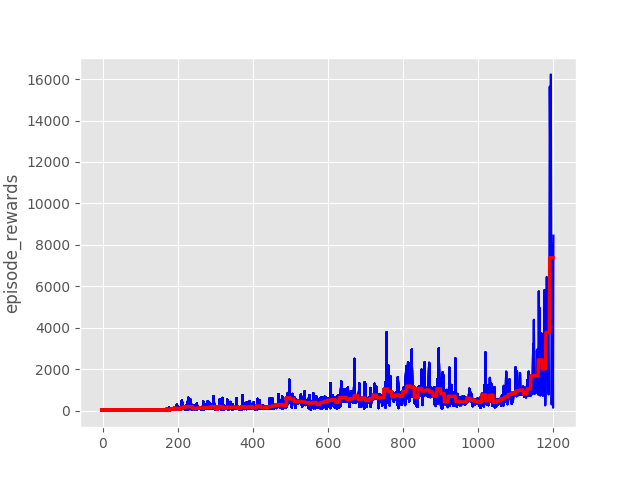
\includegraphics[width=0.8\textwidth]{figs/ch2/cartpole-epoch-1200}
\caption{Reward history of training A Cart-Pole Agent. (Blue line: the rewards of each time step; Red line: the rewards of every 10 time steps)}
\label{fig:cartpole-result}
\end{figure}

As shown in Fig. \ref{fig:cartpole-result}, the accumulated reward in each episode was gradually increasing and had a huge jump when it came to Episode 1200. After that, it had a satisfying ability to keep balance for a considerable period of time.

%%%%%%%%%%%%%%%%%%%%%%%%%%%%%%%%%%
\section{Vehicle Model}

A well performed vehicle model kit, Dataspeed ADAS Kit Gazebo/ROS Simulator, is adopted here.

\subsection{URDF Models}

\begin{figure}[h]
\centering
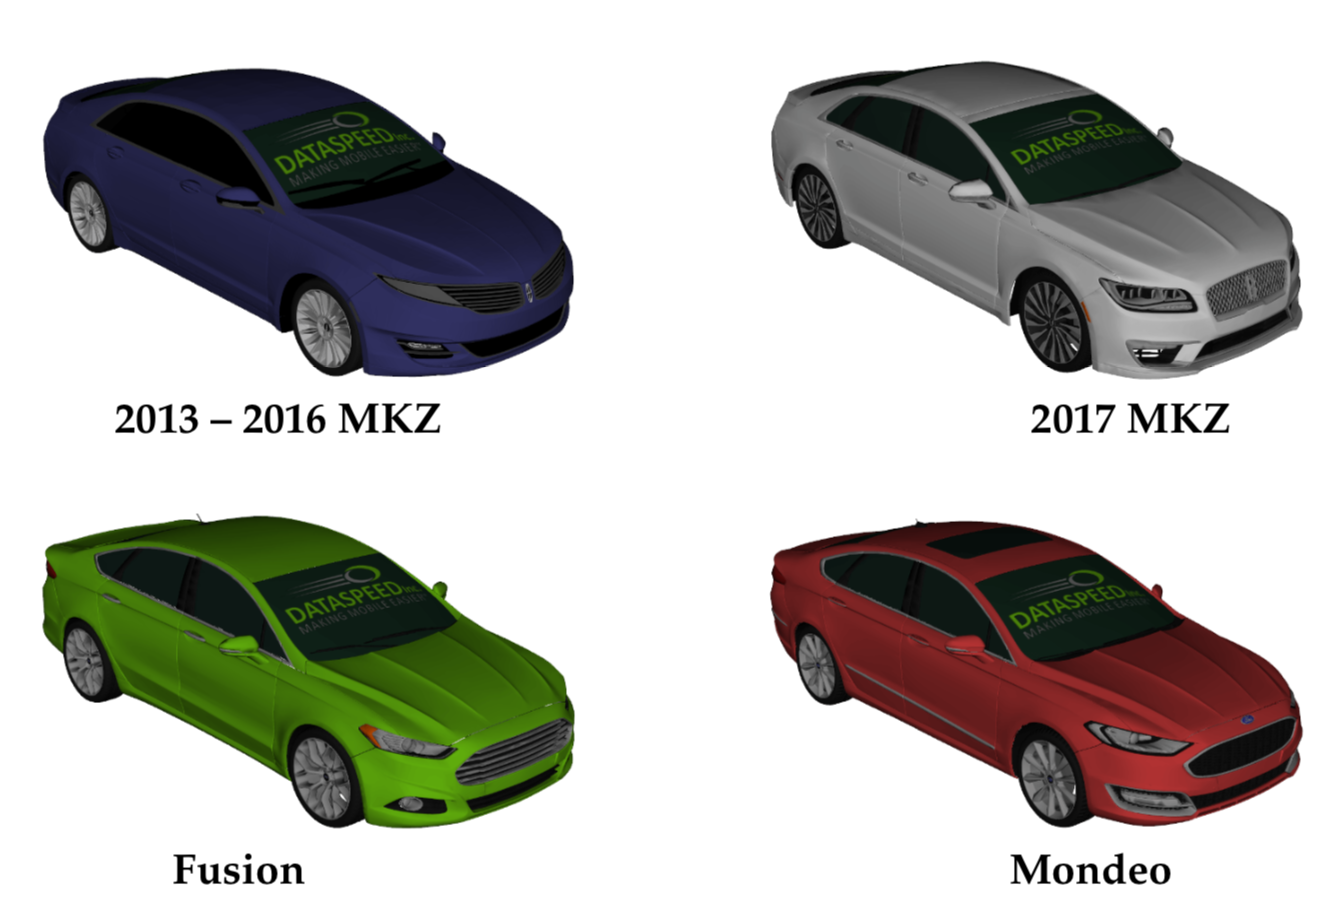
\includegraphics[width=0.8\textwidth]{figs/ch2/mkz-cover}
\caption{4 vehicle models in ADAS Kit.}
\label{mkz-models}.
\end{figure}

Four URDF models representing the different vehicles supported by the Dataspeed ADAS Kit are included in the simulation, as shown in Fig. \ref{mkz-models}. The TF trees of the simulation models are all the same, and this common TF tree is shown in Fig. \ref{fig:dataspeed}.

\begin{figure}
\centering
\begin{minipage}{.5\textwidth}
  \centering
  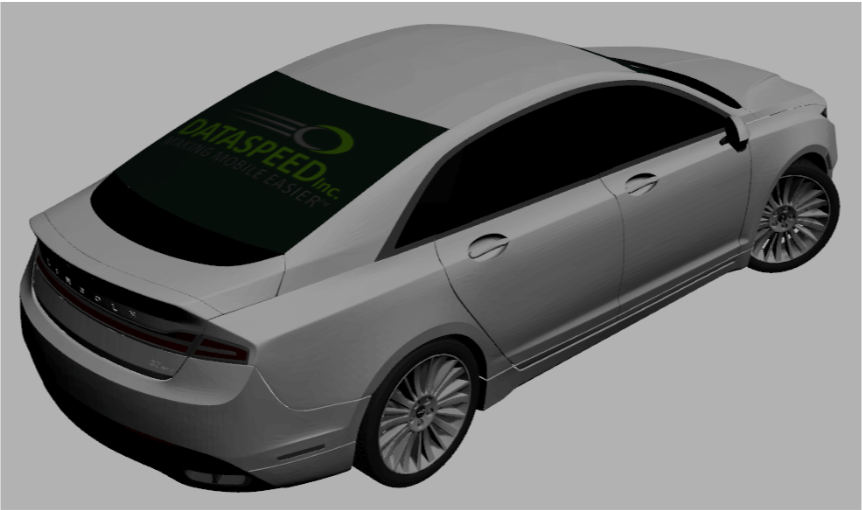
\includegraphics[width=0.9\linewidth]{figs/ch2/mkz-model}
  \label{fig:sub1}
\end{minipage}%
\begin{minipage}{.5\textwidth}
  \centering
  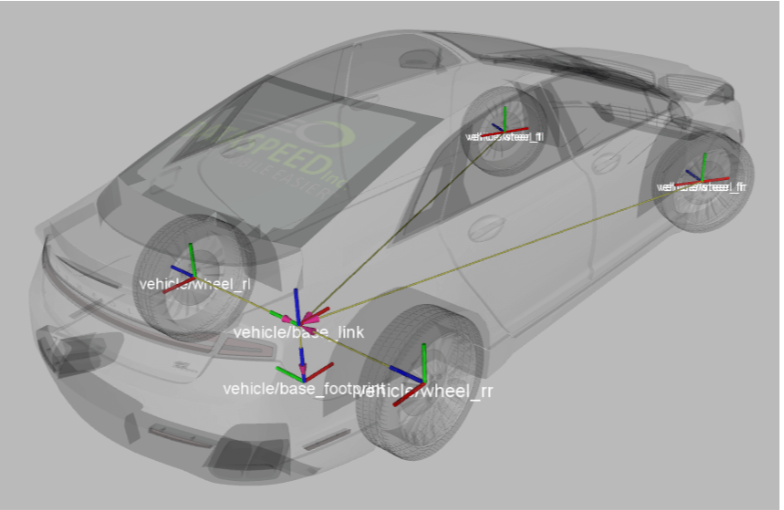
\includegraphics[width=0.82\linewidth]{figs/ch2/mkz-tf-tree}
  \label{fig:sub2}
\end{minipage}
\caption{Simulation model and corresponding TF tree.}
\label{fig:dataspeed}
\end{figure}

\subsection{Simulated CAN Message Interface}

The simulator emulates the CAN message interface to the real ADAS Kit. Therefore, there are only two ROS topics used to interact with the simulated vehicle: $can\_bus\_dbw / can\_tx$ to send CAN messages to the vehicle, and $can\_bus\_dbw / can\_rx$ to receive feedback data from the vehicle. These topics and their corresponding message types are listed in Table \ref{table:dbw1}.

\begin{table}[h!]
\centering
\begin{tabular}{c c} 
 \hline
 Topic Name & Msg Type \\ [0.5ex] 
 \hline
 $~<name>/can\_bus\_dbw/can\_rx$ & $can\_msgs/Frame$  \\ 
 \hline
 $~<name>/can\_bus\_dbw/can\_tx$ & $can\_msgs/Frame$ \\ [1ex] 
 \hline \\
\end{tabular}
\caption{CAN message topics to interact with simulated ADAS Kit.}
\label{table:dbw1}
\end{table}

The simulator only implements a subset of the complete Dataspeed CAN message specification. The supported command messages are listed in Table \ref{table:dbw3}, and the supported report messages are listed in Table \ref{table:dbw3}. See the ADAS Kit datasheets for complete CAN message information.

\begin{table}[h!]
\centering
\begin{tabular}{c c} 
 \hline
 Command Msg & CAN ID \\ [0.5ex] 
 \hline
 Brake & 0x060 \\ 
 \hline
 Throttle &0x062 \\
  \hline
 Steering & 0x064 \\
 \hline
 Gear & 0x066 \\  [1ex] 
 \hline \\
\end{tabular}
\caption{Command CAN messages supported by the ADAS Kit simulator.}
\label{table:dbw2}
\end{table}

\begin{table}[h!]
\centering
\begin{tabular}{c c c} 
 \hline
Report Msg & CAN ID & Data Rate \\ [0.5ex] 
 \hline
Brake & 0x061 & 50 Hz \\
Throttle & 0x063 &  50 Hz \\
Steering & 0x065 & 50 Hz \\
Gear & 0x067 & 20 Hz \\
Misc & 0x069 & 50 Hz \\
Wheel Speed & 0x06A & 100 Hz \\
Accel & 0x06B & 100 Hz \\
Gyro & 0x06C & 100 Hz \\
GPS1 & 0x6D & 1 Hz \\ 
GPS2 & 0x6E & 1 Hz \\
GPS3 & 0x6F & 1 Hz \\
Brake Info & 0x074 & 50 Hz \\ [1ex]
 \hline \\
\end{tabular}
\caption{Report CAN messages supported by the ADAS Kit simulator.}
\label{table:dbw3}
\end{table}


\subsection{Simulating Multiple Vehicles}

The parameters of the ADAS Kit Gazebo simulation are set using a single YAML file. This section describes the options and formatting of the YAML file.

To simulate multiple vehicles simultaneously, simply add more dictionaries to the array in the YAML file. Below is an example:

\begin{lstlisting}[language=XML]
- vehicle1: 
x: -2.0
y: 0.0
color: red
model: mkz
year: 2017

- vehicle2:
x: 0.0
y: 2.0
color: green
model: fusion
\end{lstlisting}

This would spawn two vehicles: one red 2017 MKZ with model name $\textbf{vehicle1}$ spawned at $(0.0, -2.0, 0.0)$ and one green 2013 Fusion with model name $\textbf{vehicle2}$ spawned at $(0.0, 2.0, 0.0)$. Both vehicles would have the default values of the parameters not set in the individual dictionaries.



%\bibliographystyle{plainnat}				%Uncomment this if you want a bibliography on each chapter
%\markright{\textit{Bibliography}}
%\renewcommand{\chaptername}{}
%\bibliography{my_references}

%\vfill


\chapter{System Design}

% Overview

Current autonomous vehicles use the same architecture as the Urban DARPA Challenge vehicles did \cite{DARPA2009} \cite{FullyAD} \cite{BerthaDrive2014} \cite{PROUD2014}. This architecture comprises three main processing modules, described below and illustrated in Fig. \ref{fig:std-archi}.

\begin{figure}[h]
\centering
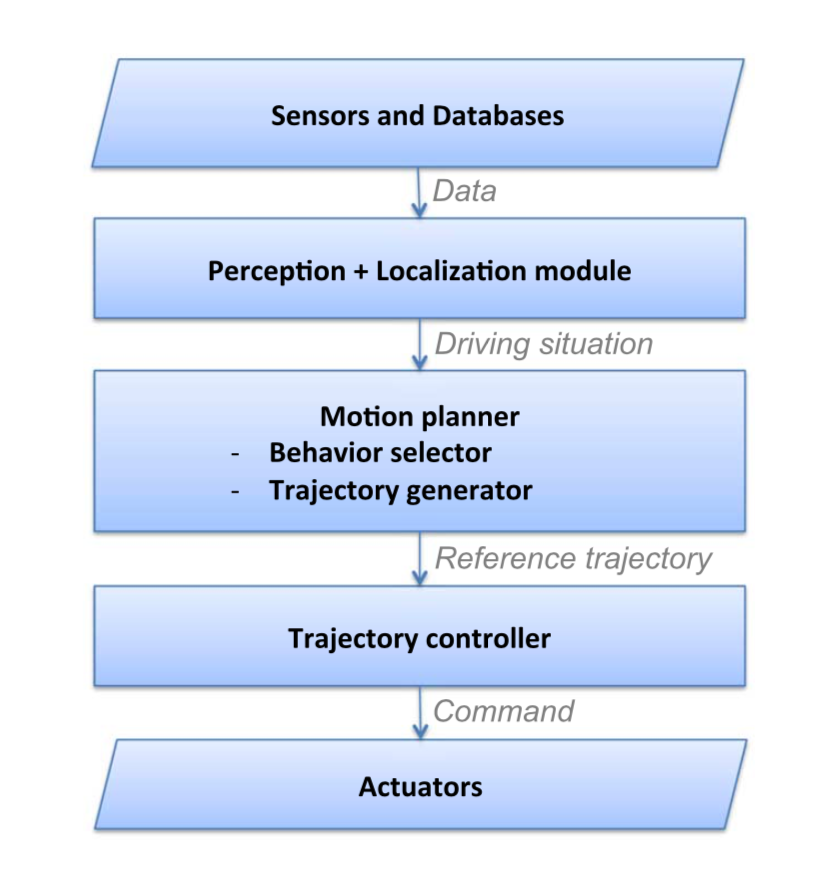
\includegraphics[width=0.5\textwidth]{figs/ch3/standard-architecture}
\caption{Standard Architecture of Autonomous Vehicle.}
\label{fig:std-archi}
\end{figure}

\begin{itemize}
\item The "Perception + Localization" module combines data received from sensors and digital maps to estimate some relevant features representing the driving situation (e.g. position of other vehicles, road geometry).
\item The "Motion planner" selects the appropriate high-level behavior (e.g. car following, lane changing) and generates a trajectory corresponding to that behavior.
\item The "Trajectory controller" computes the steering and acceleration commands with the objective to follow the reference trajectory as closely as possible. These commands are sent to the actuators.
\end{itemize}

This architecture has been successfully used in the field of terrestrial robotics for decades. Our autonomous driving framework inherits the most of it and replaces the motion planner with a trained driver model, which will be described in detail in Chapter 4.

The driver model can be designed independently and can be modified at any time without impacting the performance of the other. This feature is particularly useful if one wants to adjust the car's driving style over time: the driver model can learn continuously, or be replaced, without having to readjust any other module. One could also imagine extending the architecture in Fig. \ref{fig:proposed-architecture} to take advantage of cloud-based computing and learn new models based on data collected from millions of drivers.

\begin{figure}[h]
\centering
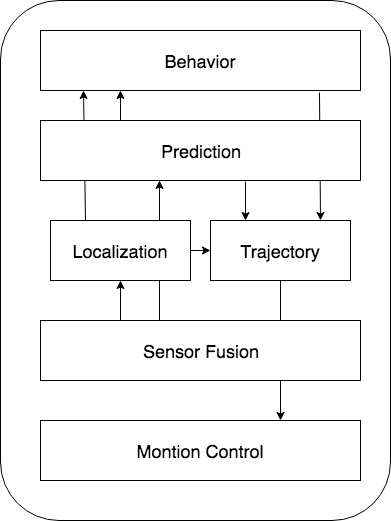
\includegraphics[width=0.5\textwidth]{figs/ch3/architecture}
\caption{Standard Architecture of Autonomous Vehicle Control.}
\label{fig:proposed-architecture}
\end{figure}

The framework proposed above is general and can be applied to a variety of driving scenarios. We will implement and test it for the longitudinal and lateral control of an autonomous vehicle during lane keeping and lane changing. In this scenario, the commanded input is the acceleration and steering of the vehicle. The system is aiming for constructing at least the following modules or functions.

% Topics
\begin{itemize}
\item \textbf{Path following} Detecting and determining a path/lane to follow, and following it.
\item \textbf{Lane and obstacle detection} Detecting driving lanes and obstacles to successfully navigate them.
\item \textbf{ACC} Detect a leading vehicle or a  trailing vehicle and maintain a safe distance and speed.
\item \textbf{Adaptive braking} Braking system adapts braking to different driving conditions to improve response time, overall safety, etc.
\end{itemize}

%%%%%%%%%%%%%%%%%%%%%%%%%%%%%%%%%%%%%%%%%%%
\section{Motion Planner}

%%%%%%%%%%%%%%%%%%%%%%%%%%%%%%%%%%%%%%%%%%%
\subsection{Longitudinal Control:  Adaptive Cruise Control}

We define the following variables to represent the relative motion of the autonomous vehicle (referred to as the "ego vehicle") and the vehicle located ahead or behind in the same lane as the autonomous vehicle (referred to as the "preceding vehicle" or the "trailing car").

\begin{itemize}
\item $\epsilon = [d_t, v_t]$ is the state of the ego vehicle at time \textit{t}, where $d_t \in R^+$ is the longitudinal position of the ego vehicle in a road-aligned coordinate system, and $v_t \in R^+$ is the longitudinal velocity of the ego vehicle.
\item $\epsilon = [d_t^p, v_t^p]$ is the state of the preceding vehicle at time \textit{t}, where $d_t \in R^+$ is the longitudinal position of the preceding vehicle in a road-aligned coordinate system, and $v_t \in R^+$ is the longitudinal velocity of the preceding vehicle.
\item $\epsilon = [d_t^t, v_t^t]$ is the state of the trailing vehicle at time \textit{t}, where $d_t \in R^+$ is the longitudinal position of the trailing vehicle in a road-aligned coordinate system, and $v_t \in R^+$ is the longitudinal velocity of the trailing vehicle.
\item $z_t =  [d_t^{pr}, d_t^{tr}, v_t^p, v_t^t, v_t^t]$ are the features representing the current driving situation at time \textit{t} , to be used by the driver model to generate an appropriate acceleration command. $d_t^{pr} = d_t^p - d_t$ is the relative distance to the preceding vehicle and $d_t^{tr} = d_t^t - d_t$ is the relative distance to the preceding vehicle.
\end{itemize}

At each time step \textit{t} , the driver model generates an acceleration command. This acceleration command is used by the trajectory generator to compute a target velocity as a reference. The controller solves a constrained optimization problem over the prediction horizon , and generates a planned velocity sequence which guarantees the safety of the vehicle.

%%%%%%%%%%%%%%%%%%%%%%%%%%%%%%%%%%%%%%%%%%%
\subsection{Lateral Control: Lane Change Control}

We define a one-dimensional array with boolean values to represent the lateral position of the autonomous vehicle in a 3-lane highway scenario.

\begin{itemize}
\item $lane = [false, true, false]$ , for example, represents the vehicle locates at the middle lane at time \textit{t}.
\end{itemize}

\begin{figure}[h]
\centering
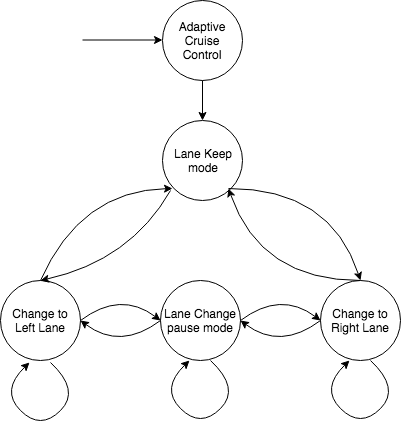
\includegraphics[width=0.7\textwidth]{figs/ch3/state-machine}
\caption{The finite state machine for lateral motion control.}
\label{fig:fsm}
\end{figure}

At each time step \textit{t} , the driver model, with the information above together with the other vehicle in its left and right lanes, generates a change lane or a keep lane command. The proposed algorithm will encourage the ego vehicle to change to a different lane neighboring to it when the target lane has better driving condition and to keep the current lane if else. To avoid conflict two lane changing commands which are too close, the lateral control would stay the current state for a period of time for the lane change to finish. Within the time period, new lane change or lane keep commands would be ignored. By this idea, it becomes a rule-based controller, sometimes referred to as "?nite state machine (FSM)", as shown in Fig. \ref{fig:fsm}. FSM has its own advantages, including:

\begin{enumerate}
\item \textbf {Clear in structure:} the controller is based on "if-then-else" logic, which is explicitly readable, so that the controller's behavior can be relatively easily predicted; 
\item \textbf {Easy to calibrate:} a FSM usually has a ?nite number of parameters, so that it is easy to calibrate and optimize;
\item \textbf {More reliable:} A well-calibrated FSM is usually more reliable, compared to some other frameworks, e.g., based on function approximation techniques as used in machine learning-based approaches.  
\end{enumerate}

%%%%%%%%%%%%%%%%%%%%%%%%%%%%%%%%%%%%%%%%%%%
\section{Trajectory Generator}

\subsection{Trajectory Planning}

The proposed Trajectory Generator is used to generate a safe and comfortable path (with an appropriate speed and acceleration) from an initial position towards a destination, while complying with a global route and map. Our method aims to resolve local path planning problems based on a global route and map. The global route is obtained by the high precision navigation system, and the map is downloaded from the Internet. The map is composed of a set of waypoints on the road edges and topology that describes the relationships between connected roads, as shown in Fig. \ref{fig:center-line}. The process by which the map is obtained falls outside the scope of this thesis. Therefore, the maps used in this paper are predefined in our simulations.

\begin{figure}[h]
\centering
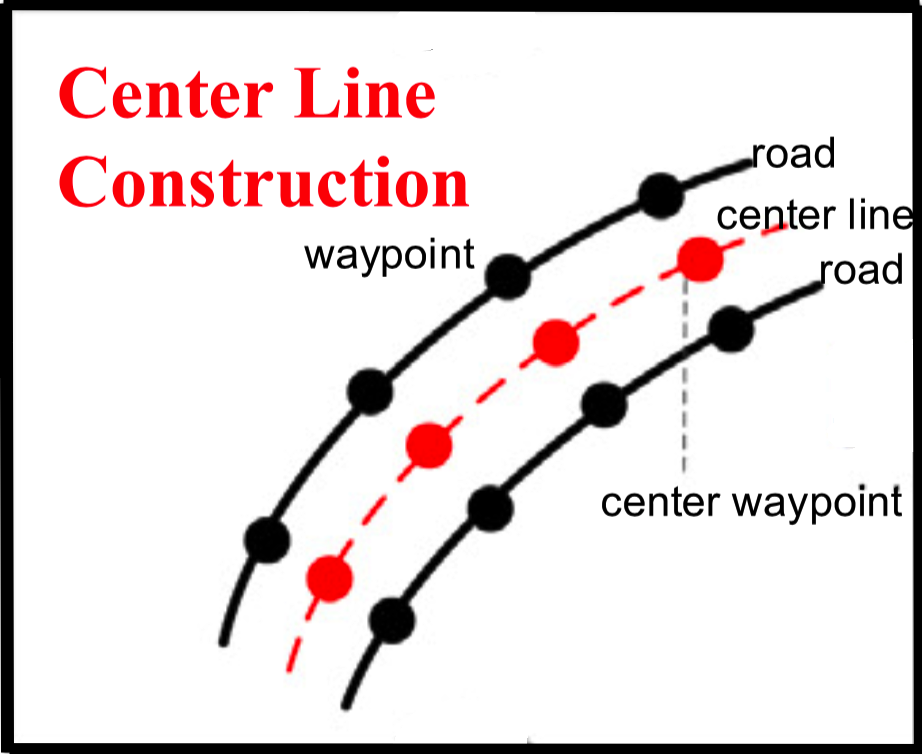
\includegraphics[width=0.5\textwidth]{figs/ch3/center-line}
\caption{The global route and the waypoints.}
\label{fig:center-line}
\end{figure}

The dynamic path planning process includes three stages: center line construction, path candidate generation, and path selection. These are performed on the basis of perceived information. The center line of the road is constructed from the center waypoints, which are several waypoints captured from the map and aligned to the center line of the lane, using the method of cubic spline fitting. The path candidates, which are also described by the cubic spline, are generated by adjusting the lateral offset to the center line using the information for the current vehicle position, speed, and direction in a road-aligned coordinate system. During path selection, the costs of static safety, comfortability, and dynamic safety are taken into account, and are combined with information on road edges, and static and moving obstacles for selecting the optimal path. Our method provides not only the selected path, but also the appropriate speed for the vehicle maneuvering system. In this project, the proposed dynamic path planning algorithm is executed 50 times per second, and a new path is generated from the current vehicle position at every time step. 

\subsection{A road-aligned coordinate system: Frenet Coordinate}

As we have mentioned several times in the previous section, a road-aligned coordinate system is needed to have a better view on the global and local trajectories. A well known one is the Frenet coordinate, which asserts invariant tracking performance under the action of the special Euclidean group $SE(2) := SO(2) \times \mathbb{R}^2$. Here, we will apply this coordinate system in order to be able to combine different lateral and longitudinal cost functionals for different tasks as well as to mimic human-like driving behavior on the highway. As depicted in Fig. \ref{fig:traj-generation}, the moving reference frame is given by the tangential and normal vector $\overrightarrow{t_r}$, $\overrightarrow{n_r}$ at a certain point of some curve referred to as the center line in the following. This center line represents either the ideal path along the free road, in the most simple case the road center, or the result of a path planning algorithm for unstructured environments \cite{Frenet2008}. Rather than formulating the trajectory generation problem directly in Cartesian Coordinates $\overrightarrow{x}$, we switch to the proposed dynamic reference frame and seek to generate a one-dimensional trajectory for both the root point $\overrightarrow{r}$ along the center line and the perpendicular offset \textit{d} with the relation

\begin{figure}[h]
\centering
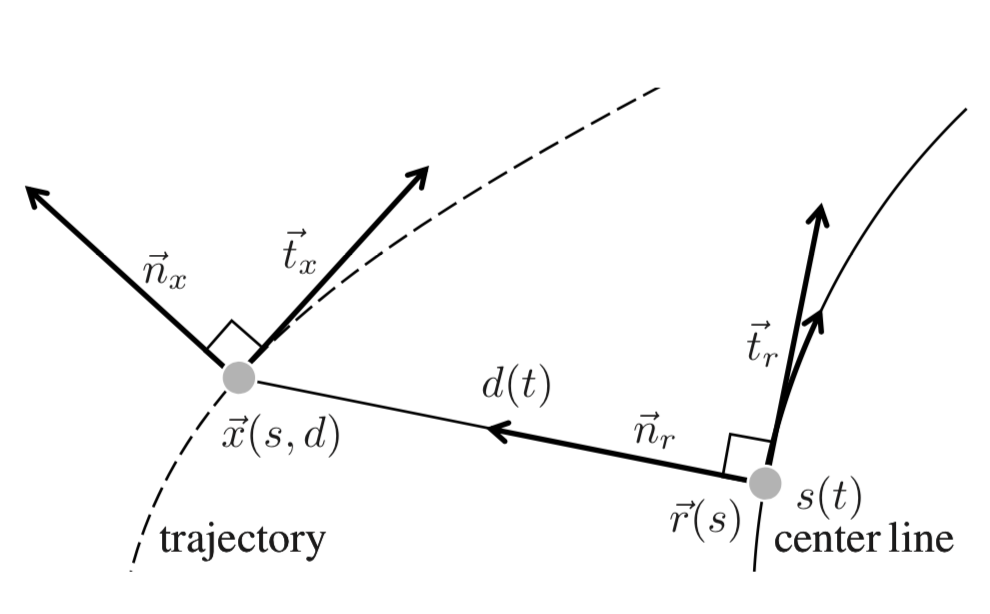
\includegraphics[width=0.5\textwidth]{figs/ch3/traj-generation}
\caption{Trajectory generation in Frenet coordinate.}
\label{fig:traj-generation}
\end{figure}

\subsubsection{Frenet Coordinates}


Frenet Coordinates are a way of representing position on a road in a more intuitive way than traditional $(x,y)$ Cartesian Coordinates. With Frenet coordinates, we use the variables $s$ and $d$ to describe a vehicle's position on the road. The $s$ coordinate represents distance along the road (also known as longitudinal displacement) and the $d$ coordinate represents side-to-side position on the road (also known as lateral displacement). Imagine a curvy road like in Fig. \ref{fig:curve-in-cartesian} with a Cartesian coordinate system laid on top of it.

\begin{figure}[h]
\centering
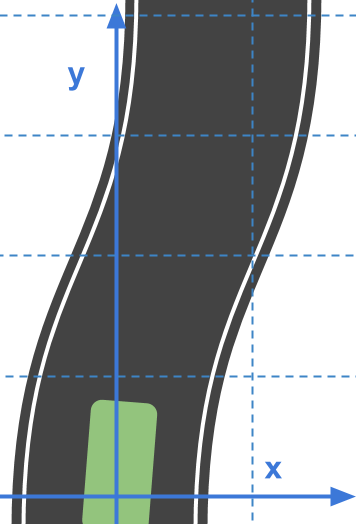
\includegraphics[width=0.25\textwidth]{figs/ch3/curve-in-cartesian}
\caption{A curve road in Cartesian coordinate.}
\label{fig:curve-in-cartesian}
\end{figure}

Using these Cartesian coordinates, we can try to describe the path a vehicle would normally follow on the road as shown in Fig. \ref{fig:curve-in-cartesian-wp}.

\begin{figure}[h]
  \centering
    \begin{minipage}{.5\textwidth}
        \centering
        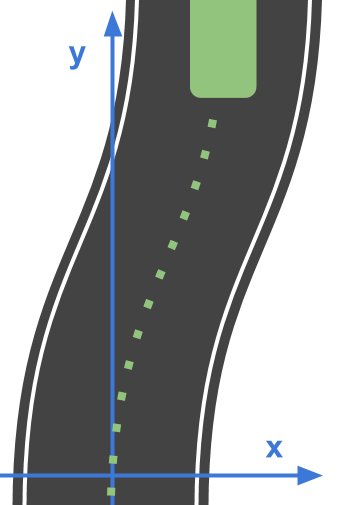
\includegraphics[height=2.4in]{figs/ch3/curve-in-cartesian-with-waypoints}
    \end{minipage}
    ~
    \begin{minipage}{.5\textwidth}
       \centering
      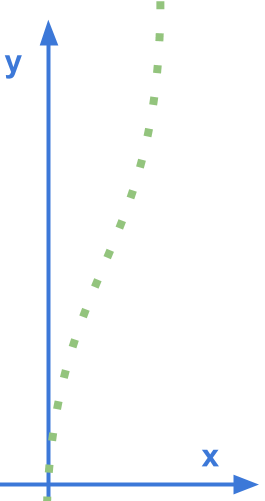
\includegraphics[height=2.4in]{figs/ch3/waypoints-in-cartesian}
     \end{minipage}
\caption{A curve road in Cartesian coordinate with waypoints.}
\label{fig:curve-in-cartesian-wp}
\end{figure}

And notice how curvy that path is. If we wanted equations to describe this motion it wouldn't be easy. Ideally, it should be mathematically easy to describe such common driving behavior. Now instead of laying down a normal Cartesian grid, we would refer to Frenet coordinate system as below in Fig. \ref{fig:curve-in-frenet}.

\begin{figure}[h]
\centering
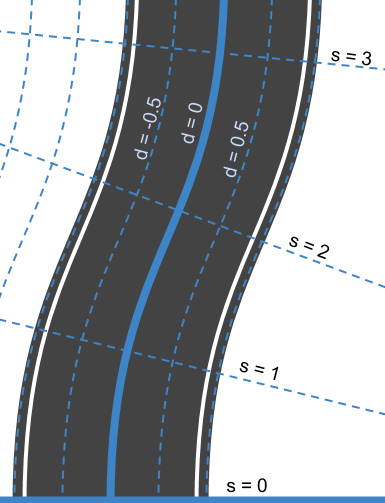
\includegraphics[width=0.25\textwidth]{figs/ch3/curve-in-frenet}
\caption{Curve in Frenet coordinate system.}
\label{fig:curve-in-frenet}
\end{figure}

Here, we've defined a new system of coordinates. At the bottom we have s=0 to represent the beginning of the segment of road we are thinking about and $d=0$ to represent the center line of that road. To the left of the center line we have negative $d$ and to the right $d$ is positive. Then a typical trajectory would look like in Fig. \ref{fig:curve-in-frenet-wp} when presented in Frenet coordinate.

\begin{figure}[h]
  \centering
    \begin{minipage}{.5\textwidth}
        \centering
        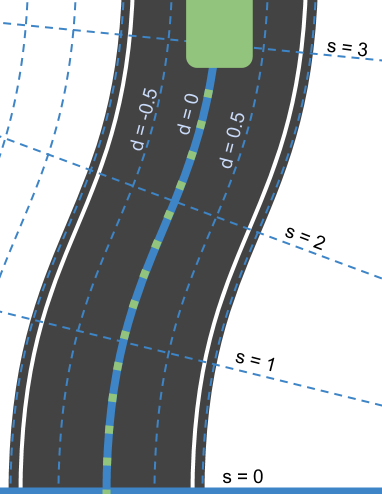
\includegraphics[height=2.4in]{figs/ch3/curve-in-frenet-with-waypoints}
    \end{minipage}
    ~
    \begin{minipage}{.5\textwidth}
       \centering
      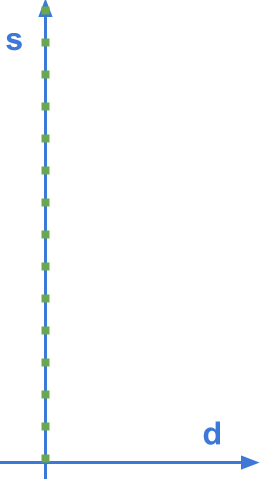
\includegraphics[height=2.4in]{figs/ch3/waypoints-in-frenet}
     \end{minipage}
\caption{A curve road in Frenet coordinate with waypoints.}
\label{fig:curve-in-frenet-wp}
\end{figure}

It looks straight! In fact, if this vehicle were moving at a constant speed of $v_0$ we could write a mathematical description of the vehicle's position as:

\begin{subequations} \label{eq:math-in-frenet}
\begin{align}
s(t) &= v_0^t \\
d(t) &= 0
\end{align}
\end{subequations}

\begin{figure}[h]
\centering
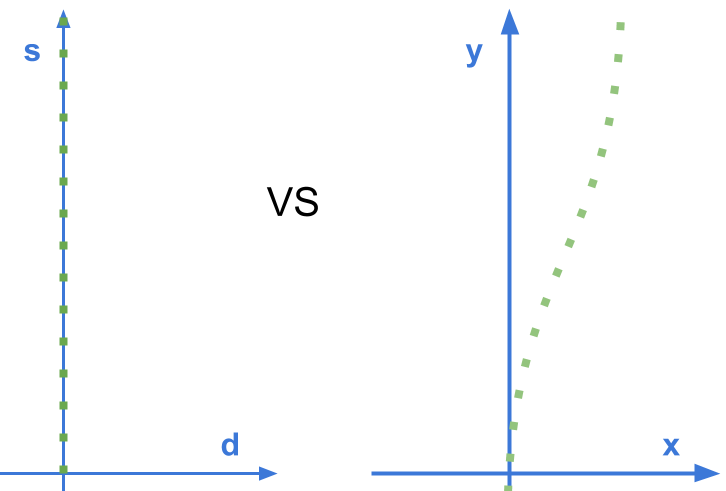
\includegraphics[height=2.8in]{figs/ch3/frenet-final}
\caption{Comparison display in Frenet and Cartesian coordinate systems.}
\label{fig:frenet-final}
\end{figure}

Straight lines are so much easier than curved ones.

\subsection{Reference path generation}

The path is the trajectory guiding the vehicle to follow a global route and avoid obstacles. The arc length $s$ indicates the traveling distance on the global route, and the offset $\rho$ can be used to measure the distance between the vehicle and the road edge.

To use the direction and curvature of the center line, it is necessary to find the position of the vehicle on the reference waypoints. We first map the vehicle position from the Cartesian coordinate system to the Frenet coordinate system, and then determine the closest point of the center line $p_0$, which has the minimum distance $\rho_{min}$. In this paper, a method combining quadratic minimization and Newton's method is used to find $p_0$.

\begin{figure}[h]
\centering
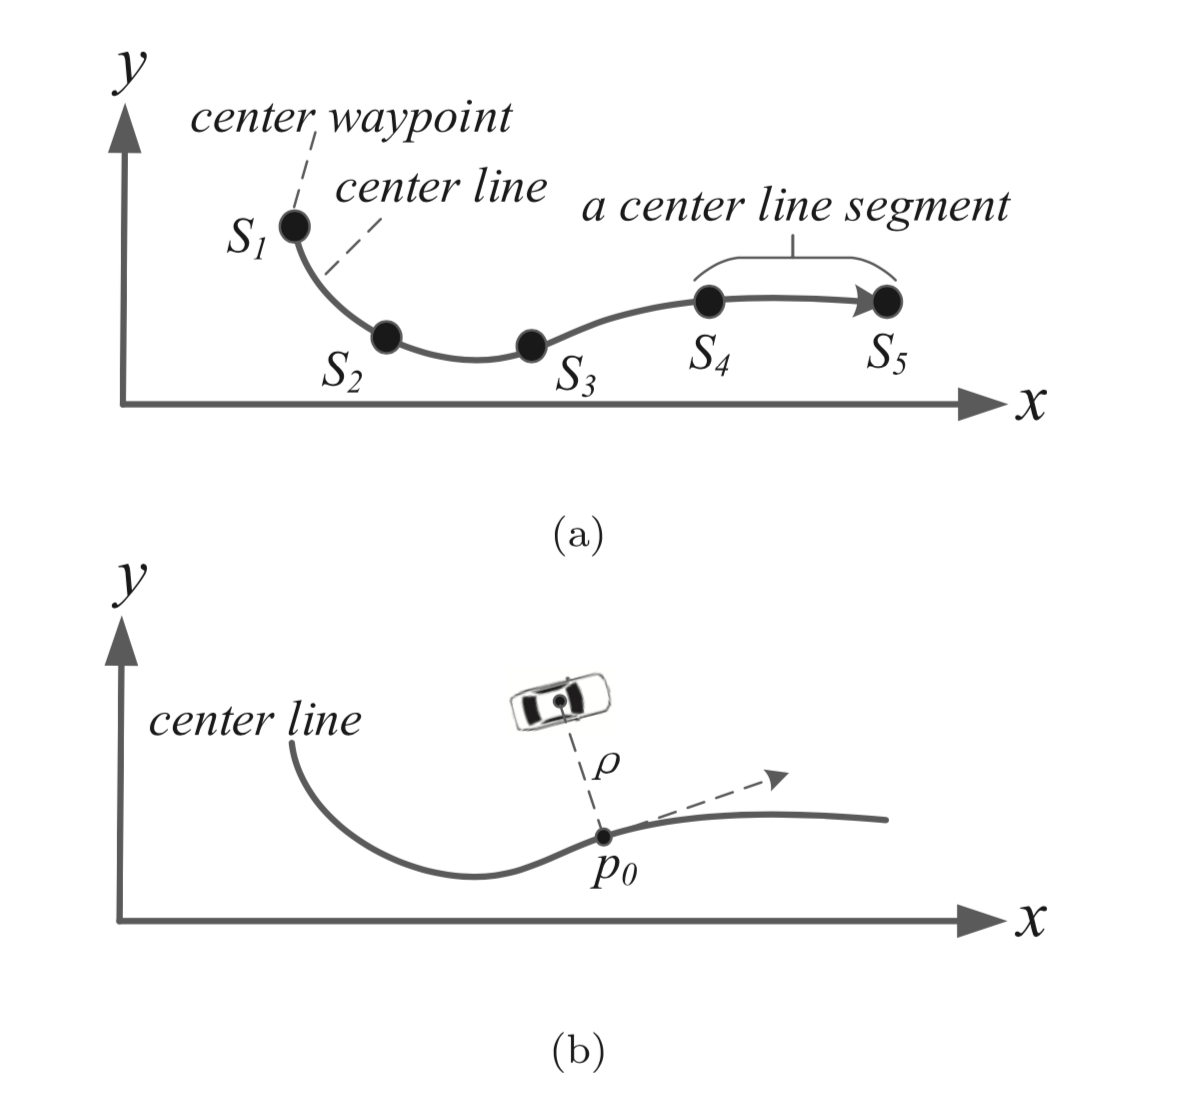
\includegraphics[height=2.8in]{figs/ch3/location-on-center-line}
\caption{Vehicle localization on the center line. (a) Center waypoints and center line segments, (b) localization on the center line.}
\label{fig:loc-line}
\end{figure}

To generate path candidates, the curvature of each path is determined by the lateral offset $d$ of the path, based on the curvature of the center line. As shown in Fig. \ref{fig:loc-line} (a), $p_{init}$ is the original point on the center line. $p_{start}$ and $p_{end}$ are the start and end points on the center line, respectively, for one step of planning. $p_{veh}$ is the start point of the vehicle. $p_1$ to $p_5$ are the end points of five path candidates, and are indicated by $r_1$ to $r_5$. It is obvious that only $r_2$; $r_4$, and $r_5$ are available and free of obstacles. The reason for this availability lies with the differences between the offset from the path candidate to the center line and the offset from the obstacle to the center line. Meanwhile, the positions of the obstacle and the vehicle on the center line can be expressed by the arc length $s$.

Path candidates are generated in the Frenet coordinate system, but path planning results must be mapped into a Cartesian coordinate system to convey to the maneuvering system. Path candidate points in the Cartesian coordinate system can be represented with respect to the arc length of the center line as Eq. (6) [43].

%%%%%%%%%%%%%%%%%%%%%%%%%%%%%%%%%%%%%%%%%%%
\section{Path Flowing}

bla

%%%%%%%%%%%%%%%%%%%%%%%%%%%%%%%%%%%%%%%%%%%
\section{Drive By Wire}

An autonomous car require that actuators that control the motion of the vehicle, can be interacted with electronically. Therefore a drive-by-wire system is needed. A drive-by-wire system replaces the mechanical systems in a traditional vehicle by using electrical/electronic (E/E) systems to perform fundamental vehicle functions.

The drive-by-wire system includes steer-by-wire, brake-by-wire and throttle-by-wire. The "by-wire" expression means that the information, from the sensor to the actuator of the different systems, is transferred electronically through wires and not by traditional hydraulic systems or mechanically through struts or shafts.

The advantage of using drive-by-wire rather than mechanical systems is that reduction of cost, moving parts and weight can be achieved. Since the steering rack can be removed, the car?s shock impact, in case of a collision, can be improved. Using an electrical based system will also increase the information flow and ease up the interconnect between different components in the car, facilitating the use of safety functions such as; ABS (anti-lock brake system), ESP (electronic stability programme), etc.

%%%%%%%%%%%%%%%%%%%%%%%%%%%%%%%%%%%%%%%%%%%
\section{Experiment}

\subsection{Lane Keep}

\begin{figure}[h]
\centering
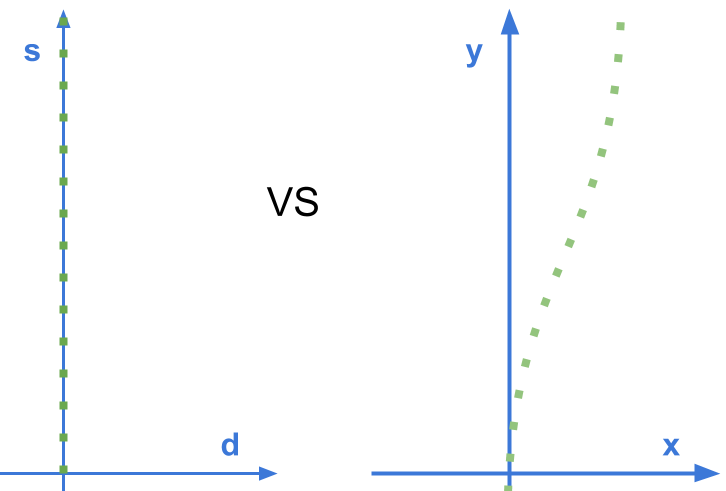
\includegraphics[height=2.8in]{figs/ch3/frenet-final}
\caption{Comparison display in Frenet and Cartesian coordinate systems.}
\label{fig:lane-keep}
\end{figure}

\subsection{Lane Change}

\begin{figure}[h]
\centering
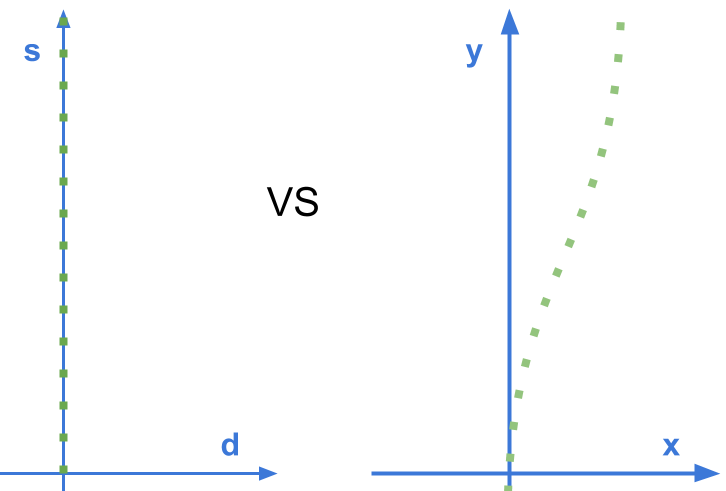
\includegraphics[height=2.8in]{figs/ch3/frenet-final}
\caption{Comparison display in Frenet and Cartesian coordinate systems.}
\label{fig:lane-change}
\end{figure}

%\bibliographystyle{plainnat}
%\markright{\textit{Bibliography}}
%\renewcommand{\chaptername}{}
%\bibliography{KL-Thesis}

%\end{flushleft}
%\vfill

\chapter{Deep Q-Learning}

With algorithms such as Q-Learning, one can learn by choosing the actions and observing their results directly in the environment. Put into an ACC context, it is possible to learn an acting policy in a simulated highway system by taking ac- tions on the cars? brakes and throttle, and observing the results. The policy obtained can be used as a longitudinal controller to safely follow a preceding vehicle.

\section{General Architecture}

Our system follows the basic RL structure. The agent performs an action $A_t$ given state $S_t$ under policy $\pi$. The agent receives the state as feedback from the environment and gets the reward $r_t$ for the action taken. The state feedback that the agent takes from sensors consists of the velocities of the neighboring vehicles $v_{veh}[]$ and the relative positions of the neighboring vehicles to the ego vehicle $dist_{veh}[]$. Possible action that agent can choose is among 4 levels of accelerations, 4 levels of decelerations and keeping the current speed. The goal of our proposed Adaptive Cruise System is to maximize the expected accumulated reward called "value function" that will be received in the future within an episode. Using the simulations, the agent learns from interaction with environment episode-by-episode. One episode starts when the vehicle and road state information are detected. The vehicle drives on a standard circular track . If the distance between the ego vehicle and the front vehicle or the behind vehicle is less than the safety distance $dist_{safe}$, it is considered as a collision event. The episode ends if at least one of the following events occurs

\begin{itemize}

\item \textbf{Collision} The ego vehicle detects the distance with the vehicle in front or behind within $dist_{safe}$.

\item \textbf{Time Out} The ego vehicle failed to finished N laps within a specific time.

\item \textbf{Finishing} The ego vehicle successfully finished N laps within a specific time.

\item \textbf{Bump} The ego vehicle is turned over for some reason.

\item \textbf{Off Lane} The ego vehicle is out of lanes.

\end{itemize}

The ego vehicle continuously detect the vehicles around itself as shown in Fig \ref{fig:highway}. The vehicle $i$ ($i$ = 0,1,...,5) do not represent any specific vehicle but a detected vehicle in that area. For example, Vehicle 0 and Vehicle 1 represent vehicles in the left lane of the ego vehicle and Vehicle 0 is behind and Vehicle 1 is in front of it. When there are multiple vehicles in the same area, only the closest is remained. When there is no vehicle there, a fake and safe vehicle would be used to maintain the state structure, which would be described in more detail later.

\begin{figure}[h]
\centering
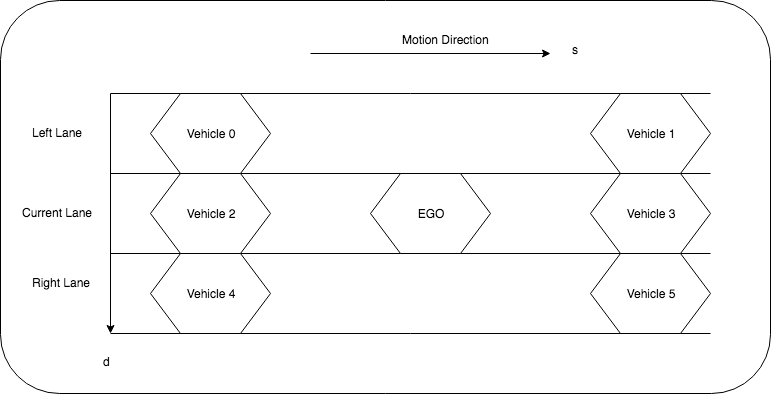
\includegraphics[width=0.5\textwidth]{figs/ch4/Highway-Display}
\caption{A general highway case display.}
\label{fig:highway}
\end{figure}

Once one episode ends, the next episode starts with the state of environment and the value function reset.


\section{Reinforcement Learning for Longitudinal Motion}

Reinforcement Learning (RL) is an interesting technique for the design of a longitudinal controller because it enables us to abstract from the complexity of car physics and dynamics that have an important computing cost. With algorithms such as Q-Learning, one can learn by choosing the actions and observing their results directly in the environment. Put into an ACC context, it is possible to learn an acting policy in a simulated highway system by taking actions on the cars? brakes and throttle, and observing the results. The policy obtained can be used as a longitudinal controller to safely follow a preceding vehicle.

To apply this RL framework, we first had to model the problem by defining the states, actions, goals and rewards. Our first approach was to use variables such as the position of a leading car and of a follower, their velocities and accelerations, etc. Clearly, this state definition put us up against the curse of dimensionality, and it became impossible to have a discrete state space precise enough to learn a valuable policy. We modified our state definition by consolidating numerous state variables. This allowed us to use a smaller discretization and to reach a better precision with only two variables. Since driving can be seen as a sequential decision problem, there is no problem in modeling it using a MDP and discrete state variables. As seen in section 7, part of our future works will be to implement techniques to better approximate the continuous aspects of the problem. For now, our discrete state space was built around a state definition containing variables similar to those used in [14] for a fuzzy logic controller, as we defined our states by the relative distance in time between two vehicles and by the difference between those distances at two consecutive steps.

As seen in Eq. (1) and Eq. (2), the time distance takes into ac- count the relative position between the two vehicles and also the velocity of the follower, while the differences of the time distance between two consecutive time steps gives a signal about the movement of the vehicles relative to each other (whether they are closing up since last step, or getting farther). The time distance is the main variable for identifying the follower?s position related to the secure distance, while the difference in time completes the Markovian signal, as it adds to the state definition an evaluation of the relative acceleration or deceleration. This relative movement between vehicles is needed to take an informed decision on the action to take at the next time step. Those actions were taken directly on the brakes or throttle (only one action per time step is chosen), closely simulating human interaction. The actions were discretized, according to a percentage of pressure on the pedal, from 0 to 100 by increments of 20.

The goal was defined as a secure distance to reach behind a pre- ceding vehicle. That distance was specified as a time range and was defined as 2 seconds (� 0.1 sec.), as it is a value often used as a se- cure distance in today?s ACC systems [2]. To reach the goal, we set the rewards accordingly, with a positive reward given when the ve- hicle was located in the specified time range. We also set negative rewards when wandering too far or too close from the time ratio we were looking for. The behavior the agent was supposed to learn was to reach the secure distance specified as the goal, and to stay in that range for as long as possible.

Those elements were put together in a RL framework, and the policy obtained, learned in a simulated environment, formed the core of our longitudinal controller. The environment, a simulated highway system built in previous work, featured complex car physics and dynamics as described in [9]. Since the simulation environment was using continuous time, we had to define the time interval at which action decisions would be taken. The action chosen at the specified time frame would be taken for the whole frame. To observe an accurate behavior of the vehicle, we had to set the time step between each action decision to a small value (50 milliseconds). But in such conditions, the observation of real vehicle acceleration needed many consecutive acceleration actions, a behavior that could not be learned in a decent time with normal state space exploration. To overcome this problem, we had to use a heuristic to speed up learning. The heuristic specified that every time the car was behind the desired time ratio, the best acceleration action known from experience was taken. By ignoring in that case the braking actions, this action selection technique directed rapidly the agent towards more rewarding locations of the state space.

\begin{figure}[h]
\centering
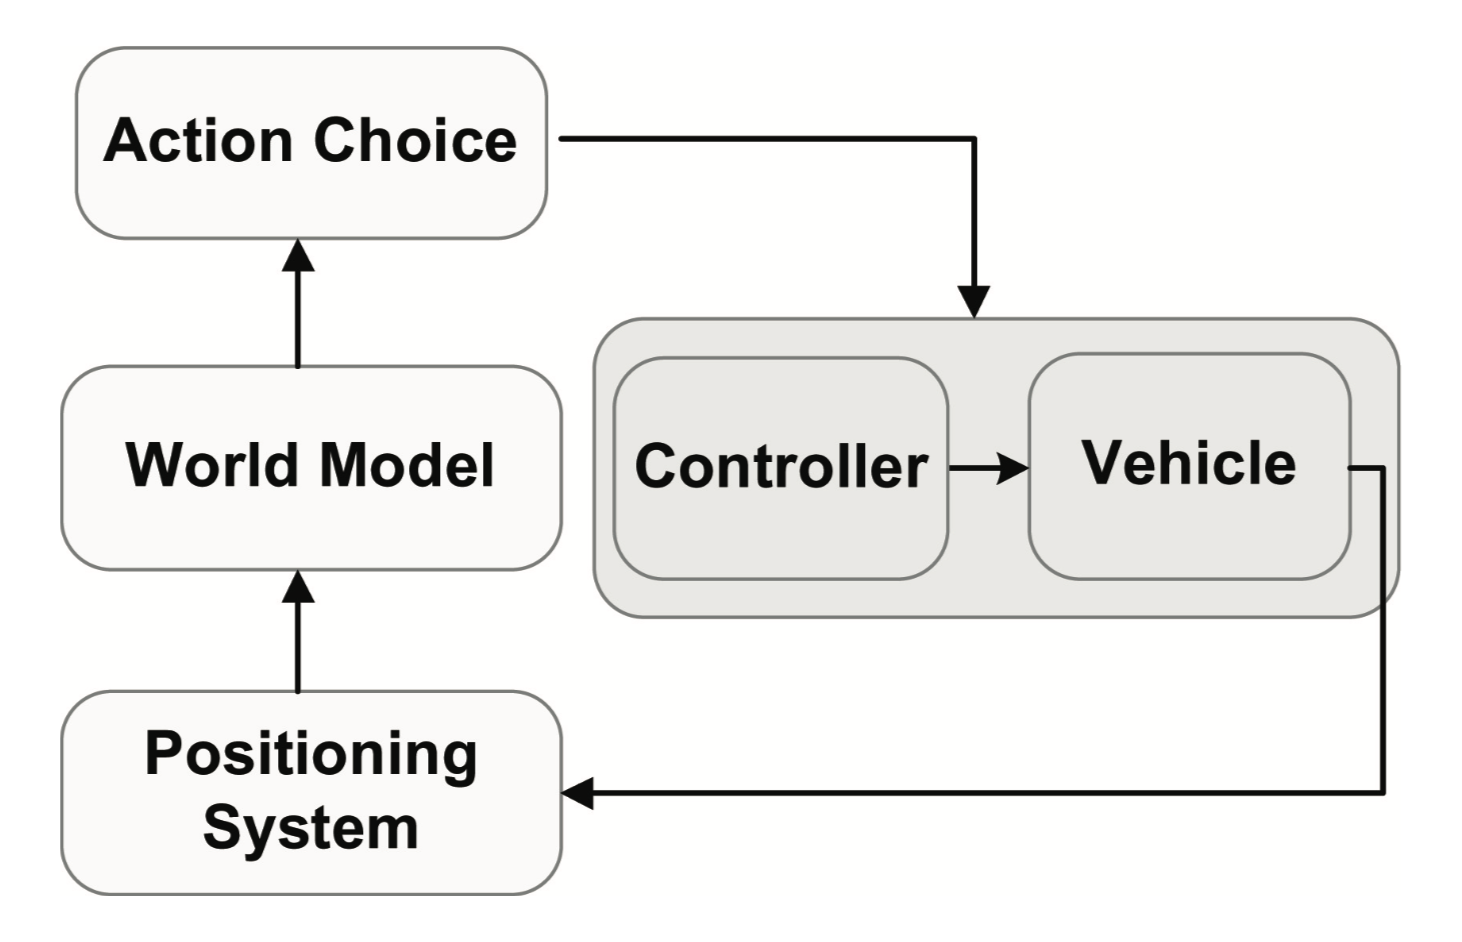
\includegraphics[width=0.5\textwidth]{figs/ch4/acc-drl}
\caption{Reinforcement applied on ACC system.}
\label{fig:acc-rl}
\end{figure}

Put into context, Figure 3 shows that using RL simplifies the de- sign of a longitudinal controller. The closed-loop controller takes as inputs the vehicle?s state as described earlier, and selects the appropriate action according to the policy that was learned. Such a technique is obviously simpler than the complex mathematical analysis needed to predict precise car physics and dynamics for act- ing, as our controller basically hides in a black box vehicle physics and dynamics. It is possible for the agent to learn the optimal behavior by taking driving actions and observing their results on the time distance and its difference between two time steps. In the next section, we will show results obtained by using this policy for longitudinal vehicle control. As drivers spend a great amount of their time in heavy traffic, such systems could reduce the risk of rear-end collisions and protect the drivers mentally by relieving them from stressful driving. (Source: [67])

\section{Reinforcement Learning for Lateral Motion}

Lateral motion control without longitudinal motion control hardly exists. Besides parking another good example of low speed combined longitudinal and lateral control is the traffic jam assist system. At speeds between zero and 40 or 60 km/h (depending on OEMs), the traffic jam assist system keeps pace with the traffic flow and helps to steer the car within certain constraints. It also accelerates and brakes autonomously. The system is based on the functionality of the adaptive cruise control with stop \& go, extended by adding the lateral control of steering and lane guidance. The function is based on the built-in radar sensors, a wide-angle video camera and the ultrasonic sensors of the parking system.


In this section, we describe the design of the Management layer and, more precisely, the design of the policy to select the most efficient and safest lane for each vehicle according to their current state and action.

Lane changes are stressful maneuvers for drivers, particularly during high-speed traffic flows.


\section{Q Learning}

Q-learning is one of the popular RL methods which searches for the optimal policy in an iterative fashion. Basically, the Q-value function $q_{\pi} (s, a)$ is defined as

\begin{equation}
q_\pi(s,a) = \mathbb{E}_\pi \left[ \sum _{k=0}^{\infty} \gamma ^k r_{t+k+1} | S_t = s, A_t = a \right]
\end{equation}

For the given state s and action a, where $r_t$ is the reward received at the time step t. The Q-value function is the expected sum of the future rewards which indicates how good the action $a$ is given the state $s$ under the policy of the agent $\pi$. The contribution to the Q-value function decays exponentially with the discounting factor $\pi$ for the rewards with far-off future. For the given Q-value function, the greedy policy is obtained as

\begin{equation} \label{eq:402}
\pi(s) = arg \max_a q_{\pi} (s, a) 
\end{equation}

One can show that for the policy in Eq. \ref{eq:402}, the following Bellman equation should hold,

\begin{equation}
q_\pi(s,a) = \mathbb{E}_\pi [r_{t+1} + \gamma \max_a q_\pi(S_{t+1},a) | S_t = s, A_t = a]
\end{equation}

In practice, since it is hard to obtain the exact value of $q_{\pi}(s, a)$ satisfying the Bellman equation, the Q-learning method uses the following update rule for the given one step backups $S_t$, $A_t$, $r_{t+1}$, $S_{t+1}$;

\begin{equation}
q_\pi(S_t,A_t) \gets q_\pi(S_t,A_t) + \alpha \left[r_{t+1} + \gamma \max_a q_\pi(S_{t+1},a) - q_\pi(S_t,A_t)\right]
\end{equation}

However, when the state space is continuous, it is impossible to find the optimal value of the state-action pair $q_{\pi} (s, a)$ for all possible states. To deal with this problem, the DQN method was proposed, which approximates the state-action value function q(s, a) using the DNN, i.e., $q(s, a) = q_\theta(s, a)$ where $\theta$ is the parameter of the DNN. The parameter $\theta$ of the DNN is then optimized to minimize the squared value of the temporal difference error $\delta_t$

\begin{equation} \label{eq:delta-1}
\delta_t = r_{t+1} + \gamma \max_{a^ \prime} q_\theta(S_{t+1},a^ \prime) - q_\theta(S_t,A_t)
\end{equation}

For better convergence of the DQN, instead of estimating both $q(S_t,A_t)$ and $q(S_{t+1},a^ \prime)$ in  Eq. (4.5), we approximate $q(St,At)$ and $q(S_{t+1},a^ \prime)$ using the Q-network and the target network parameterized by $\theta$ and $\theta^{\prime}$, respectively. The update of the target network parameter $\theta^{\prime}$, is done by cloning Q-network parameter $\theta$, periodically. Thus, Eq. \ref{eq:delta-1} becomes

\begin{equation}
\delta_t = r_{t+1} + \gamma \max_{a^ \prime} q_{\theta^{\prime}}(S_{t+1},a^ \prime) - q_\theta(S_t,A_t)
\end{equation}

To speed up convergence further, replay memory is adopted to store a bunch of one step backups and use a part of them chosen randomly from the memory by batch size. The backups in the batch is used to calculate the loss function L which is given by

\begin{equation}
L = \sum_{t\in B_{replay}}\delta_t^2
\end{equation}

where $B_{replay}$ is the backups in the batch selected from replay memory. Note that the optimization of parameter $\theta$ for minimizing the loss $L$ is done through the stochastic gradient decent method.



One of the most basic and popular methods to estimate action-value functions is the \emph{Q-learning} algorithm. It is model-free online off-policy algorithm, whose main strength is that it is able to compare the expected utility of the available actions without requiring a model of the environment. Q-learning works by learning an action-value function that gives the expected utility of taking a given action in a given state and following a fixed policy thereafter.

A value function estimates what is good for an agent over the long run. It estimates the expected outcome from any given state, by summarizing the total amount of reward that an agent can expect to accumulate into a single number. Value functions are defined for particular policies.

The \emph{state value function} (or V-function), is the expected return when starting in state $s$ and following policy $\pi$ thereafter~\citep{Sutton1998RL},
%
\begin{equation}
V^\pi(s) = \mathbb{E}_\pi \left[R_t | s_t = s \right]
\end{equation}

The \emph{action value function} (or Q-function), is the expected return after selecting action $a$ in state $s$ and then following policy $\pi$,
%
\begin{equation}
q^\pi(s,a) = \mathbb{E}_\pi \left[ R_t | s_t = s, a_t = a \right]
\end{equation}

The \emph{optimal value function} is the unique value function that maximizes the value of every state, or state-action pair,
%
\begin{eqnarray}
Q^*(s,a) & = & \max\limits_\pi Q^\pi(s,a), \forall s \in \mathcal{S}, a \in \mathcal{A}
\end{eqnarray}

An \emph{optimal policy} $\pi^*(s,a)$ is a policy that maximizes the action value function from every state in the MDP,
%
\begin{equation}
    \pi^*(s,a) = \argmax_\pi Q^\pi(s, a)
\end{equation}

The update rule uses action-values and a built-in max-operator over the action-values of the next state in order to update $Q(s_t, a_t)$ as follows,

\begin{equation}
Q(s_t,a_t) \gets Q(s_t,a_t) + \alpha \left[r_{t+1} + \gamma \max_a Q(s_{t+1},a) - Q(s_t,a_t)\right]
\end{equation}

The agent makes a step in the environment from state $s_t$ to $s_{t+1}$ using action $a_t$ while receiving reward $r_t$. The update takes place on the action-value $a_t$ in the state $s_t$ from which this action was executed. This version of Q-learning works well for tasks with a small a state-space, since it uses arrays or tables with one entry for each state-action pair.

In this project the policy is using the \textbf{$\epsilon$-greedy} policy:

\begin{itemize}

    \item \textbf{$\epsilon$-greedy.} Selects the best action for a proportion
        $1 - \epsilon$ of the trials, and another action is randomly selected (with
        uniform probability) for a proportion,
        
        \begin{equation}
            \pi_{\epsilon}(s) = \left\{
             \begin{array}{lr}
                 \pi_{\textrm{rand}}(s,a) & \text{if } rand() < \epsilon\\
                 \pi_{\textrm{greedy}}(s,a) & \text{otherwise}
             \end{array}
           \right.
        \end{equation}

        where $\epsilon \in [0, 1]$ and $rand()$ returns a random number from a uniform distribution $\in [0, 1]$.

\end{itemize}

\section{Policy Representation}

A policy is a mapping between a state space S and an action space $A$, i.e., $\pi(s) : S \to A$. For our framework, $S$ is a continuous space that describes the state of the ego vehicle and neighboring vehicles. The action space $A$ is represented by a 27 sized 1D discrete space where each action specifies a behavior the ego vehicle could do. The following sections provide further details about the policy representation.

\subsection{State}

A state $s$ consists of features describing the state of the ego vehicle and relative positions and velocities with its neighboring vehicles. The state is represented by its pose q and velocity q?, where q records the positions of the center of mass of each link with respect to the root and q? records the center of mass velocity of each link. The terrain features, $T$ , consist of a 1D array of samples from the terrain height- field, beginning at the position of the root and spanning 10 m ahead. All heights are expressed relative to the height of the terrain immediately below the root of the character. The samples are spaced 5 cm apart, for a total of 200 height samples. Combined, the final state representation is 283-dimensional. Figure 5 and 6 illustrate the character and terrain features.

\subsection{Actions}

A total of 27 controller parameters serve to define the available policy actions. These include specifications of the target spine curvature as well as the target joint angles for the shoulder, elbow, hip,

\subsection{Reward Function}

Unlike video games, the reward should be appropriately defined by a system designer in Adaptive Cruise System. As mentioned, the reward function determines the behavior of the adaptive cruise. Hence, in order to ensure the reliability of the adaptive cruise control, it is crucial to use the properly defined reward function. In our model, there is conflict between two intuitive objectives for cruise control; 1) collision should be avoided no matter what happens and 2) the vehicle should get out of the risky situation quickly. If it is unbalanced, the agent becomes either too conservative or reckless. Therefore, we should use the reward function which balances two conflicting objectives. Taking this into consideration, we propose the following reward function

\begin{equation} \label{eq:reward-func}
r_t = \alpha * vel_{ego} + \beta * (s_{ego} - s_{behind}) + r
\end{equation}

where $v_t$ is the velocity of the vehicle at the time step $t$, decel is difference between $v_t$ and $v_{t1}$ and 1(x = y) has a value of 1 if the statement inside is true and 0 otherwise. The first term ?(?(pedposx ? vehposx)2 + ?)decel in the reward function prevents the agent from braking too early by giving penalty proportional to squared distance between the vehicle and pedestrian. It guides the vehicle to drive without deceleration if the pedestrian is far from the vehicle. On the other hand, the term ?(?vt2 + ?)1(St = bump) indicates the penalty that the agent receives when the accident occurs. Note that this penalty is a function of the vehicle?s velocity, which reflects the severe damage to the pedestrian in case of high velocity at collision. Without such dependency on the velocity, the agent would not reduce the speed in situation when the accident is not avoidable. The constants $\alpha$, $\beta$, $\phi$ and $\psi$ are the weight parameters that controls the trade-off between two objectives.

\subsection{Relay Memory}

In reinforcement learning (RL), the agent observes a stream of experiences and uses each experience to update its internal beliefs. For example, an experience could be a tuple of (state, action, reward, new state), and the agent could use each experience to update its value function via TD-learning. In standard RL algorithms, an experience is immediately discarded after it?s used for an update. Recent breakthroughs in RL leveraged an important technique called experience replay (ER), in which experiences are stored in a memory buffer of certain size; when the buffer is full, oldest memories are discarded. At each step, a random batch of experiences are sampled from the buffer to update agent?s parameters. The intuition is that experience replay breaks the temporal correlations and increases both data usage and computation efficiency Lin (1992).

Combined with deep learning, experience replay has enabled impressive performances in AlphaGo Silver et al. (2016), Atari games Mnih et al. (2015), etc. Despite the apparent importance of having a memory buffer and its popularity in deep RL, relatively little is understood about how basic characteristics of the buffer, such as its size, affect the learning dynamics and performance of the agent. In practice, a memory buffer size is determined by heuristics and then is fixed for the agent.

As mentioned in the previous section, the adaptive cruise system should learn both of the conflicting objectives. However, when we train the DQN with the reward function in Eq. \ref{eq:reward-func}, we find that the learning performance is not stable since collision events rarely happen and thus there remains only a few one-step backups associated with the collisions in the replay memory. As a result, the probability of picking such one-step backups is small and the DQN does not have enough chance to learn to avoid accidents in practical learning stage. To solve this issue, we propose so called "trauma" memory which is used to store only the one-step backups for the rare events (e.g., collision events in our scenario). While the one step backups are randomly picked from the replay memory, some fixed number of backups associated with the collision events are randomly selected from the trauma memory and used for training together. In other words, with the trauma memory, the loss function $L$ is modified to

equation ... (Autonomous Braking System via Deep Reinforcement Learning)

where $B_{trauma}$ is the backups randomly picked from trauma memory. Trauma memory persistently reminds the agent of the memory on the accidents regardless of the current policy, thus allowing the agent to learn to maintain speed and avoid collisions reliably.


\section{Deep Neural Network Layer}

Many of the successes in DRL have been based on scaling up prior work in RL to high-dimensional problems. This is due to the learning of low-dimensional feature representations and the powerful function approximation properties of neural networks. By means of representation learning, DRL can deal efficiently with the curse of dimensionality, unlike tabular and traditional non-parametric methods [15]. For instance, convolutional neural networks (CNNs) can be used as components of RL agents, allowing them to learn directly from raw, high-dimensional visual inputs. In general, DRL is based on training deep neural networks to approximate the optimal policy ??, and/or the optimal value functions $V^\star$, $Q^\star$ and $A^\star$.

Although there have been DRL successes with gradient free methods [37, 23, 64], the vast majority of current works rely on gradients and hence the backpropagation algorithm [162, 111]. The primary motivation is that when available, gradients provide a strong learning signal. In reality, these gradients are estimated based on approximations, through sampling or otherwise, and as such we have to craft algorithms with useful inductive biases in order for them to be tractable.The other benefit of backpropagation is to view the optimization of the expected return as the optimization of a stochastic function [121, 46]. This function can comprise of several parts?models, policies and value functions?which can be combined in various ways. The individual parts, such as value functions, may not directly optimize the expected return, but can instead embody useful information about the RL domain. For example, using a differentiable model and policy, it is possible to forward propagate and backpropagate through entire rollouts; on the other hand, inacuracies can accumulate

Convolutional Neural Networks, or CNNs, are a special type of neural network that has a known grid-like topology. Like most other neural networks they are trained with a variant of the back-propagation algorithm. CNN's strength is pattern recognition directly from pixels of images with minimal processing. We use a convolutional network as a function mapping the preprocessed images to Q values, since the actions are highly based on what would be seen as pixel matrix.

\begin{figure}[h]
\centering
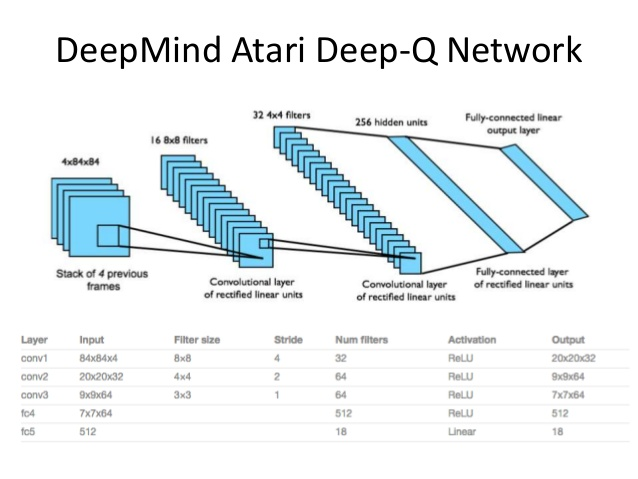
\includegraphics[width=0.5\textwidth]{figs/ch4/deepmind-atari-network}
\caption{Deep Neural Network model from DeepMind paper.}
\end{figure}



\vfill

\chapter{Results}

In this chapter, we evaluate the performance of the developed adaptive cruise and lane control system via computer simulations. It also briefly explains and discusses some characteristics of the results, whereas a more general discussion follows in the next Chapter. As described in Chapter 4, two agents with different action spaces were investigated. Agent 1 only deals with longitudinal speed control, whereas Agent 2 decides both the speed and when to change lanes.

% Furthermore, two different neural network architectures were used.

%%%%%%%%%%%%%%%%%%%%%%%%%%%%%%%%%%%%%%%%%%%%%%%%%%%%%%%%%%%%%%%%%
\section{Simulation Setup}

In simulations, we used the open source software OpenAI-Gym and ROS / Gazebo which models a highway environment in real time. We generated the environment in order to train the DQN by simulating the behaviors of the cars on highway. In the simulations, we assume that the positions and velocities of the ego vehicle's neighboring vehicles is detected in real time by the ego vehicle. In the beginning of each episode, the position of ego vehicle is set in a defined position but the velocity is initilaized with 0. The initial positions and velocities of other vehicles are initialized based on their lanes. Along with time growing, the relative positions and relative velocities among the vehicles are changing and there have chances to create several different scenarios for the DQN model to learn as below,

\begin{itemize}
\item Scenario 1: No vehicle in the ego vehicle's detecting range.
\item Scenario 2: One vehicle is detected in the same lane of the ego vehicle.
\item Scenario 3: One vehicle is detected but in a different lane of the ego vehicle.
\item Scenario 4: Vehicles are detected in both the ego's lane and the neighboring lane.
\end{itemize}

%%%%%%%%%%%%%%%%%%%%%%%%%%%%%%%%%%%%%%%%%%%%%%%%%%%%%%%%%%%%%%%%%
\section{Training for Single-lane Motion}

The Single-lane Motion means that actions here are all changing the speed. This environment with one lane as shown in Fig. \ref{fig:acc-env} would focus on training an Adaptive Cruise Control agent for the ego vehicle. The ego vehicle and the preceding vehicle would be initialized with defined the positions and headings and surely the relative position is enough safe. The dimension of the state space is set to $n = 3$ and the variables are the velocity of the ego vehicle $v_{ego}$, the longitudinal distance of the vehicles $s_{rel}$ and the relative velocity $v_{rel} = v_{pre} - v_{ego}$. To accelerate the training, they are normalized before feeding to the network.

\begin{figure}[h]
\centering
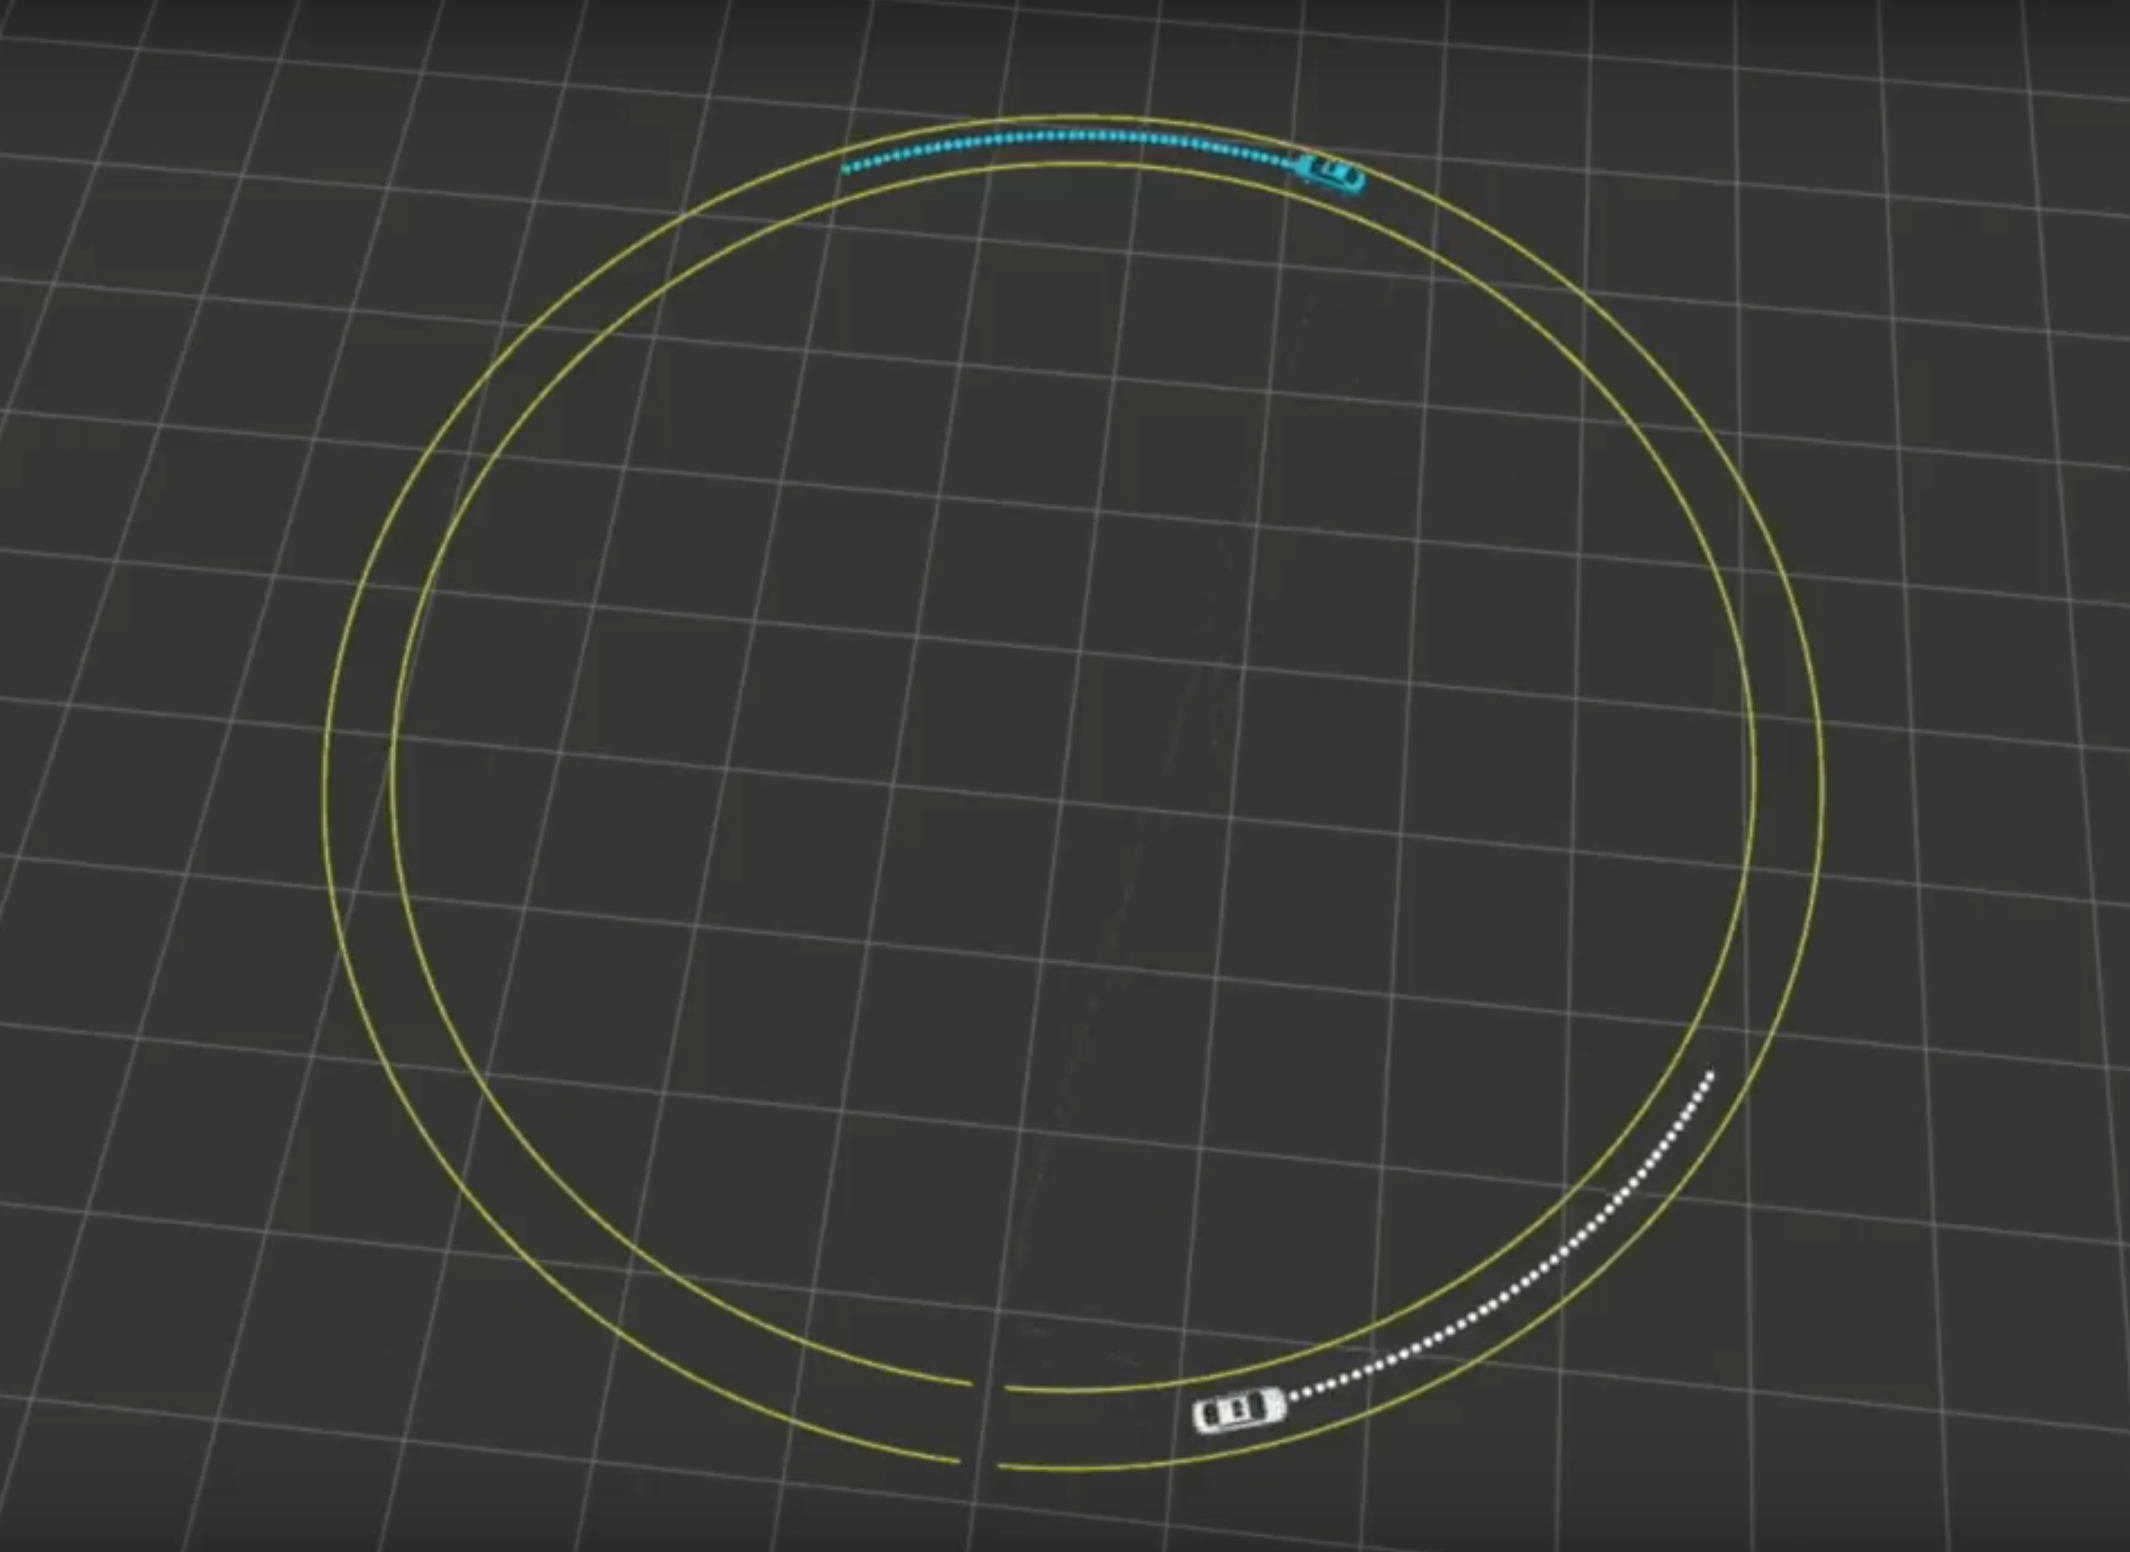
\includegraphics[width=1.0\textwidth]{figs/ch5/acc-env}
\caption{Training environment for Adaptive Cruise Control.}
\label{fig:acc-env}
\end{figure}

The neural network used for the DQN consists of the fully-connected layers with five hidden layers. RMSProp algorithm is used to minimize the loss with learning rate $\epsilon = 0.0005$. We set the size of the replay memory to 10,000. We set the replay batch size to 32. The summary of the DQN configurations used for our experiments is provided below:

\begin{itemize}
\item State buffer size: n = 3
\item Network architecture: fully-connected feed-forward network
\item Nonlinear function: leaky ReLU
\item Number of nodes for each layers : [3 (Input layer), 100, 70, 50, 70, 100, 5 (Output layer)]
\item RMSProp optimizer with learning rate 0.0005
\item Replay memory size: 10,000
\item Replay batch size: 32
\end{itemize}

The parameters are set as below,

\begin{itemize}
\item Cruise speed of the preceding vehicle is $v_{pre} = 10 m/s$ .
\item Safety distance is $dist_{safety} = 10 m$
\item $accel_{high}, accel_{low}, keep_{zero}, decel_{low}, decel_{high} = {2, 1, 0, -1, -2} m/s^2$
\end{itemize}

The reward function is as in \ref{eq:reward-func1} and we set $\alpha = 1.0$ and $\beta = 4.0$. 

\begin{itemize}
 \item $r_s$ = incremental travel distance from the last time step (we can simply use euclidean distance between the current position and the previous one since the time is short and curve road can be ignored)
 \item $r_{action}$ = \{accelerate or decelerate with 2 m/s: -1.0, accelerate or decelerate with 1 m/s: -0.5, keep the speed: 0.0\}
 \item $r_{collision}$ = \{No collision: 0.0, Collision: -100\}
\end{itemize}


\begin{figure}[h]
\centering
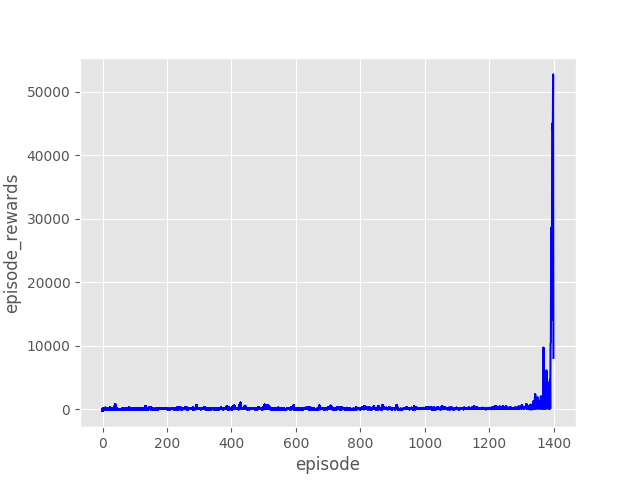
\includegraphics[width=1.0\textwidth]{figs/ch5/acc-reward}
\caption{The reward history of training for Adaptive Cruise Control.}
\label{fig:acc-reward}
\end{figure}

Fig. \ref{fig:acc-reward} provides the plot of the total accumulated rewards i.e., value function achieved for each episode. After 1400 episodes, there shows a high jump of the reward which means ACC is working and it takes forever to have a collision.

\begin{figure}[h]
\centering
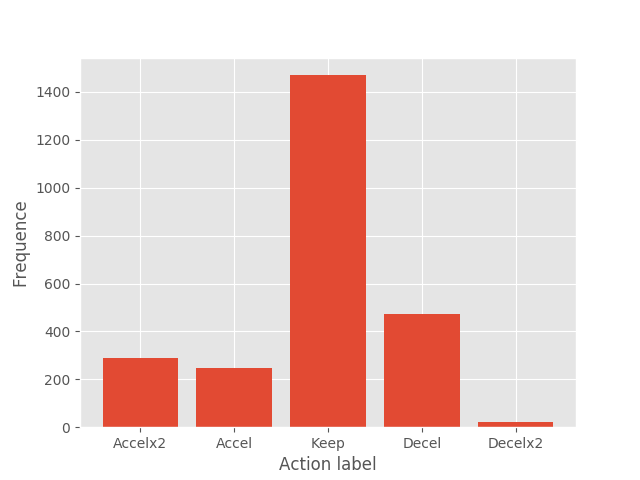
\includegraphics[width=1.0\textwidth]{figs/ch5/acc_action_distribution}
\caption{The action distribution after training.}
\label{fig:acc-action}
\end{figure}

\begin{figure}[h]
\centering
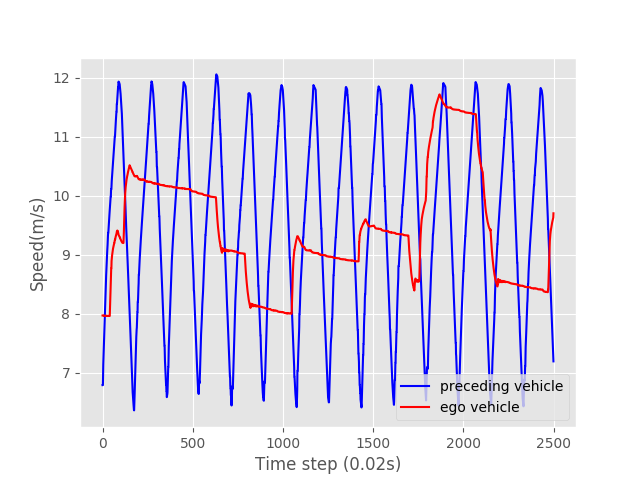
\includegraphics[width=1.0\textwidth]{figs/ch5/vel_variance}
\caption{The speed variance after training.}
\label{fig:acc-vel}
\end{figure}

To quantify the performance after 1400 episodes' training, we recorded a piece of time of driving behavior using the trained agent. As shown in Fig. \ref{fig:acc-action}, the actions are mostly chosen as ``Keep the current velocity" since our reward function penaties any speed changes. About 75\% percent actions generated by the agent during the piece of time are ``Keep velocity" (labeled as ``2"). Accordingly, the speed variance shown in Fig. \ref{fig:acc-vel} proves that the ego vehicle is closely following the speed of the preceding vehicle. The speed of the preceding vehicle is varying by 2 m/s positively or negatively around 9.5 m/s. The ego vehicle learned to maintain the same average speed but with less variance and for some duration it was relatively stable at a speed, for instance, from $200s$ to $600s$.

%%%%%%%%%%%%%%%%%%%%%%%%%%%%%%%%%%%%%%%%%%%%%%%%%%%%%%%%%%%%%%%%%
\section{Training for Multi-lane Motion}

The Multi-lane Motion means that changing the speed and changing lanes are both available as driving behaviors. This environment with two lanes as shown in Fig. \ref{fig:auto-env} would focus on training an Adaptive Cruise Control and Lane Control agent for the ego vehicle. The ego vehicle and the other two vehicles would be initialized with defined the positions and headings and surely the relative position is enough safe. The dimension of the state space is set to $n = 5$ and the variables are the velocity of the ego vehicle $v_{ego}$, the longitudinal distance of the vehicles $s_{rel}$, the relative velocity $v_{rel} = v_{pre} - v_{ego}$, the flag showing if the left lane is available $flag_{left}$ and the flag showing if the left lane is available $flag_{right}$. To accelerate the training, they are normalized before feeding to the network.

\begin{figure}[h]
\centering
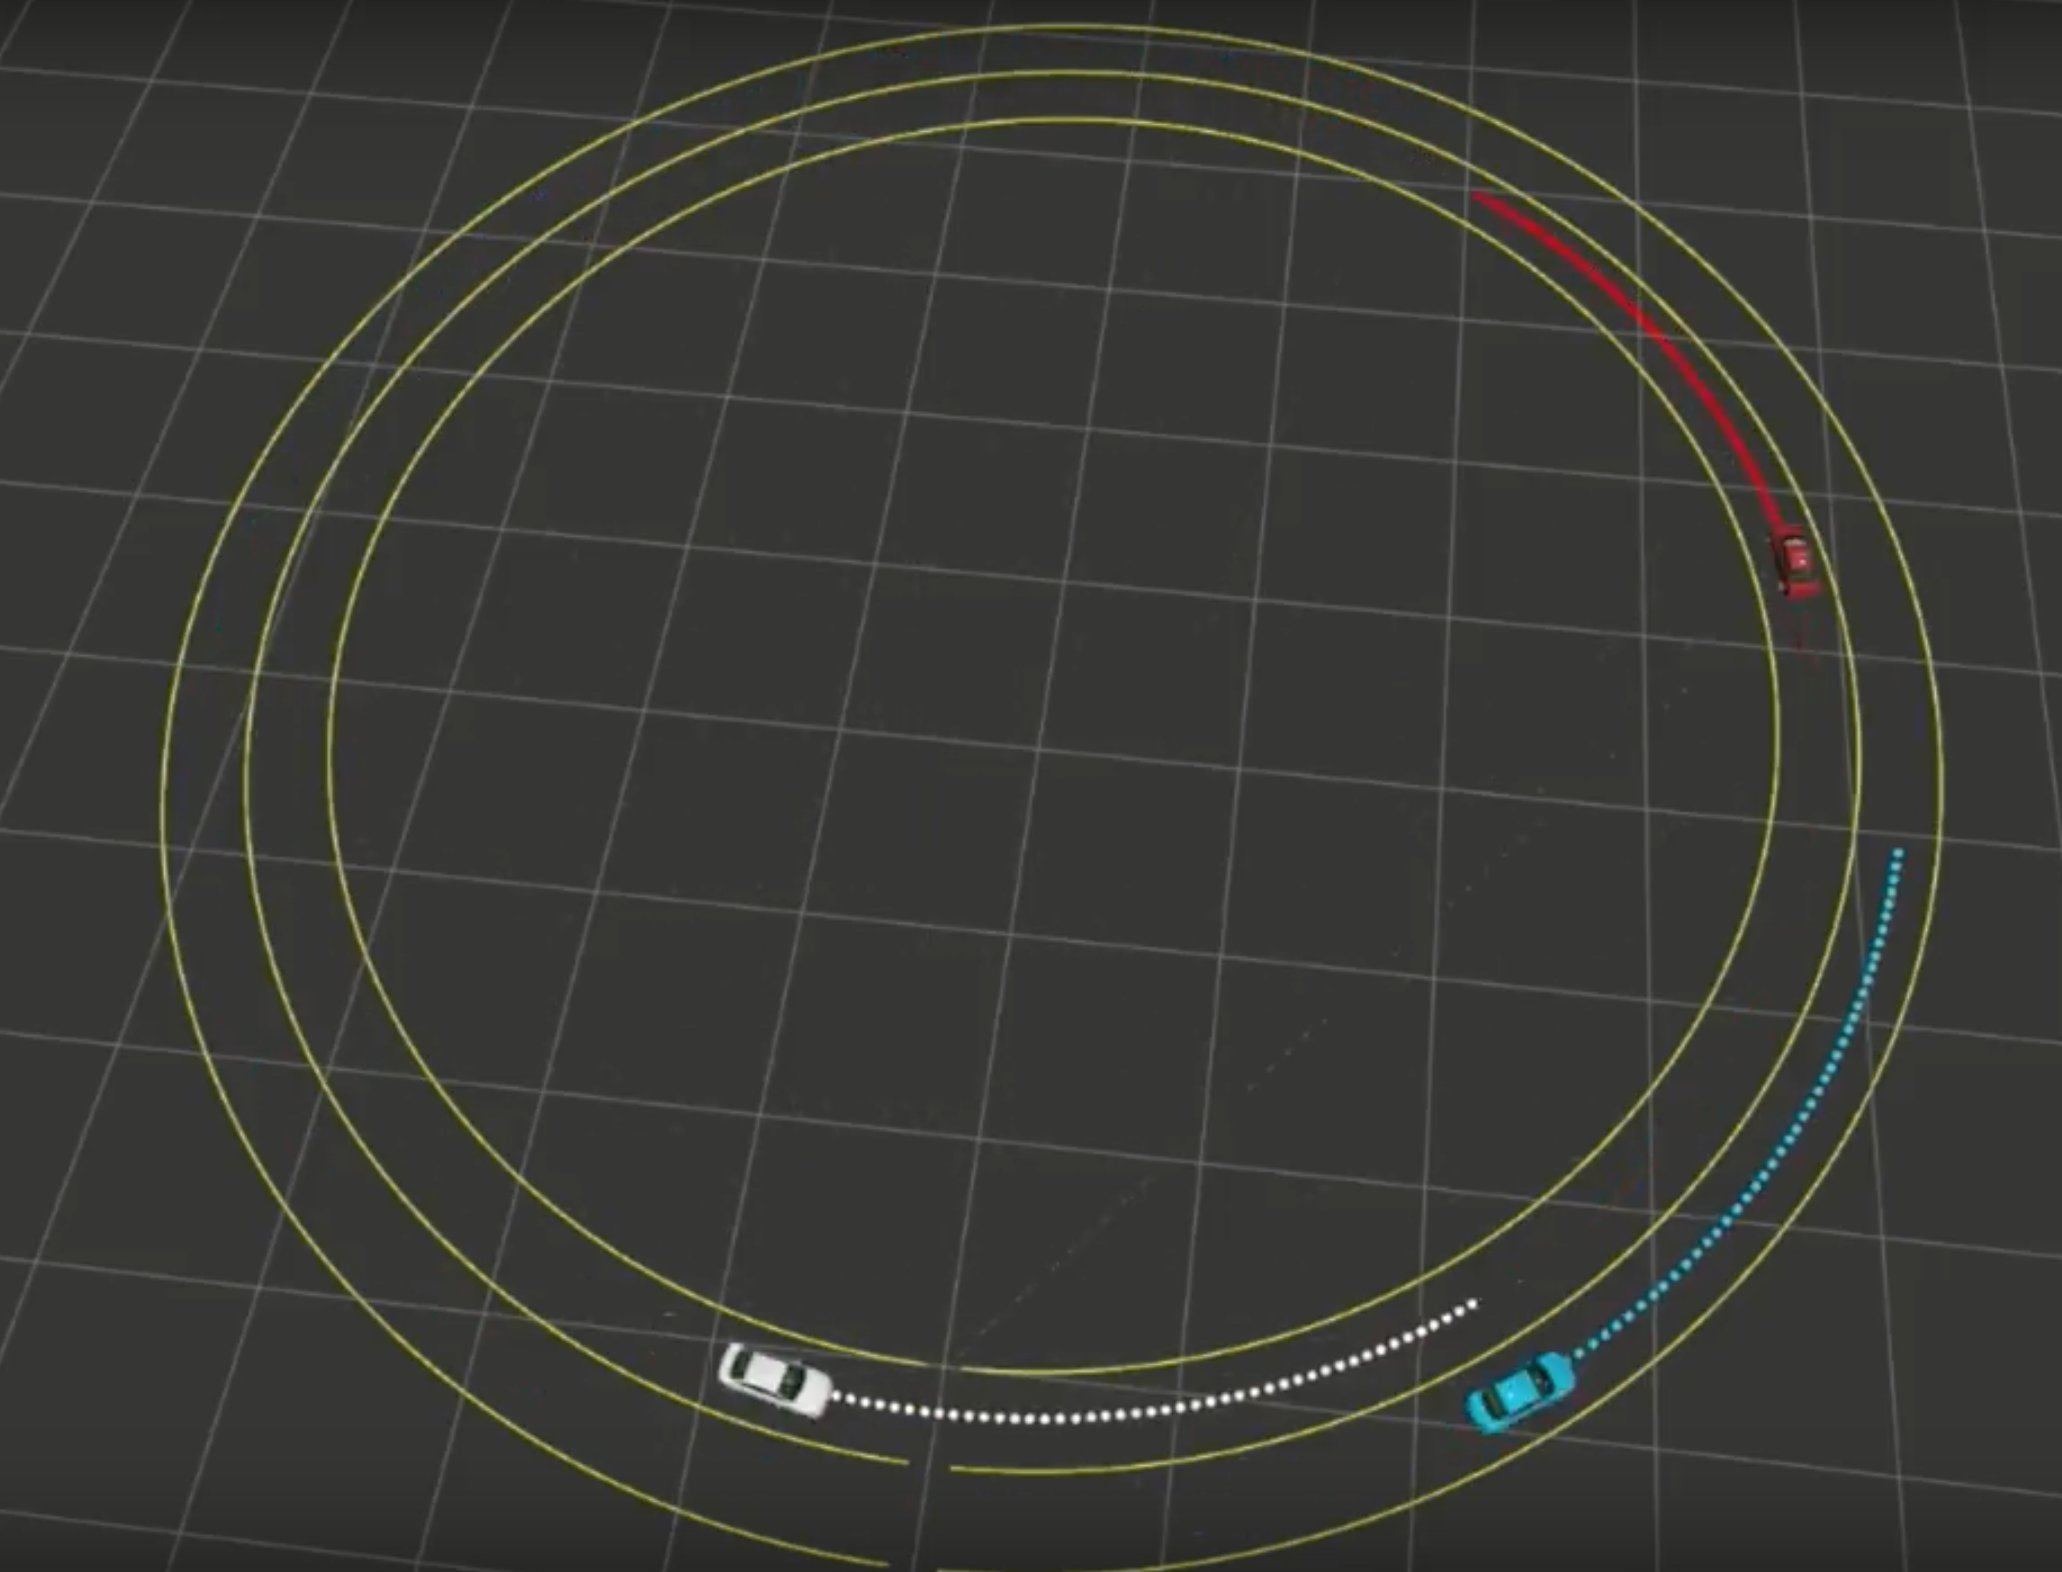
\includegraphics[width=1.0\textwidth]{figs/ch5/auto-env}
\caption{Training environment for Adaptive Cruise Control and Lane Control.}
\label{fig:auto-env}
\end{figure}

The summary of the DQN configurations used for our experiments is provided below:

\begin{itemize}
\item State buffer size: n = 5
\item Action Space size: $7 = 5 + 2$. (5 level of speed control and 2 modes of lane change)
\item Network architecture: fully-connected feed-forward network
\item Nonlinear function: leaky ReLU
\item Number of nodes for each layers : [5 (Input layer), 100, 70, 50, 70, 100, 7 (Output layer)]
\item RMSProp optimizer with learning rate 0.0005
\item Replay memory size: 10,000
\item Replay batch size: 32
\end{itemize}

The parameters are set as below,

\begin{itemize}
\item Cruise speeds in Lane 0 and 1 are $v_{lane0}, v_{lane1}$ = $6 m/s$, $5 m/s$, which means Lane 0 and 2 are Fast Lane and Slow Lane.
\item Safety distance is $dist_{safety} = 10 m$
\item $accel_{high}, accel_{low}, keep_{zero}, decel_{low}, decel_{high}$ = $2 m/s^2$, $1 m/s^2$, $0 m/s^2$, $-1 m/s^2$, $-2 m/s^2$.
\end{itemize}

The reward function is as in \ref{eq:reward-func1} and we set $\alpha = 1.0$ and $\beta = 2.0$. 

\begin{itemize}
 \item $r_s$ = travel distance from the last time step (we can simply use euclidean distance between the current position and the previous one since the time is short and curve road can be ignored)
 \item $r_{action}$ = \{accelerate or decelerate with 2 m/s: -1.0, accelerate or decelerate with 1 m/s: -0.5, keep the speed: 0.0, change lane to left or right: -1.0, change lanes when lane is not available: -3.5\}
 \item $r_{collision}$ = \{No collision: 0.0, Collision: -100\}
\end{itemize}

\begin{figure}[h]
\centering
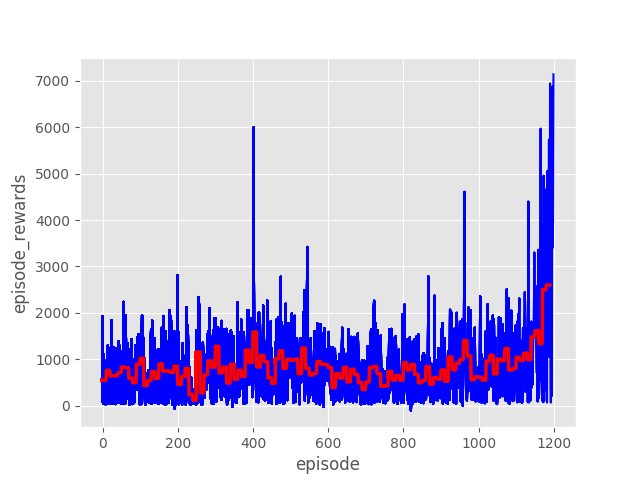
\includegraphics[width=1.0\textwidth]{figs/ch5/auto-reward}
\caption{The reward history of training for Adaptive Cruise Control and Lane Control. (Blue line: the rewards of each time step; Red line: the rewards of every 10 time steps)}
\label{fig:auto}
\end{figure}

Fig. \ref{fig:auto} provides the plot of the total accumulated rewards i.e., value function achieved for each episode. We observe that the reward increases along the episodes and high total reward is attained after 2000 episodes. Until now, the trained agent has enough ability to drive the vehicle safely in multiple lanes using speed control and lane control. Due to the training time limit, more episodes are not provided here. Since it is still exploring the boundaries in the solution space, it has potential to gain higher reward with longer training.

\begin{figure}[h]
\centering
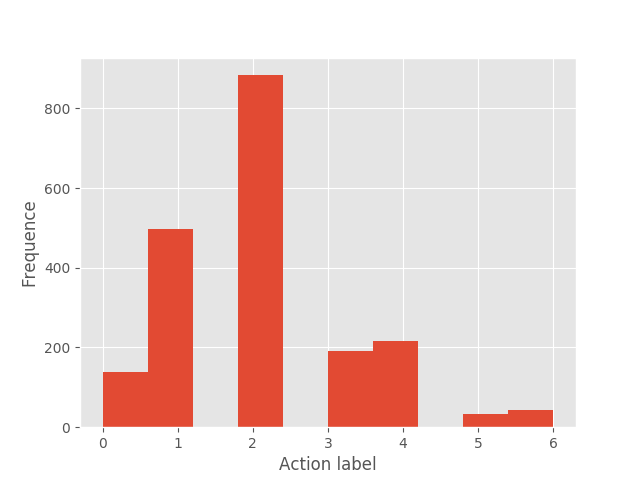
\includegraphics[width=1.0\textwidth]{figs/ch5/auto_action_distribution}
\caption{The action distribution after training.}
\label{fig:auto-action}
\end{figure}

\begin{figure}[h]
\centering
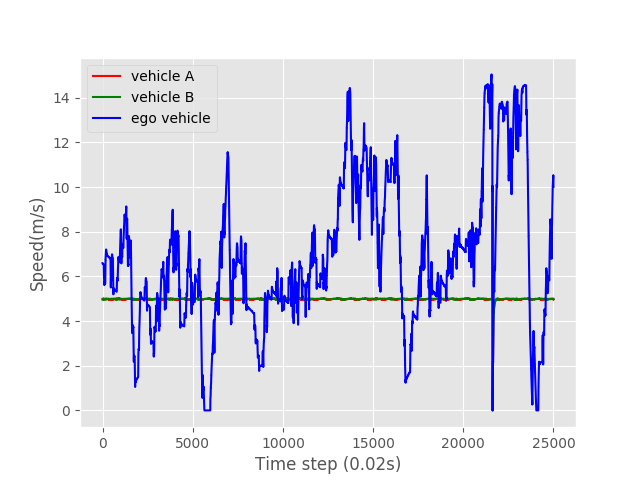
\includegraphics[width=1.0\textwidth]{figs/ch5/auto_vel}
\caption{The speed variance after training.}
\label{fig:auto-vel}
\end{figure}

Fig. \ref{fig:auto-action} indicates that the action distribution after training. Most time it will stay at constant speed by action ``Keep speed" (labeled as ``2"). The agent will rarely choose to change lanes since it would be always safe to stay in the current lane as long as the ACC is reliable. Sometimes it would take a try to change lanes and accelerate (labeled as ``0" and ``1") when no vehicle ahead in the new lane. 

As shown in Fig. \ref{fig:auto-vel}, it varied in a higher degree than that in Fig. \ref{fig:acc-vel}. That is because when lane change is available or the action space is bigger the agent takes more time to make decisions and is more likely to make mistakes. Overall, it learned to maintain an equal average speed with preceding vehicle and accelerate when changing to a new lane and there is no vehicle right ahead. With more time training, it could be expected to perform better.

\section{Main Evaluation}

Both $Agent1_{FCNN}$ and $Agent2_{FCNN}$ successfully drove the ego vehicle safely without collisions for a very long time and distance after enough training. Naturally, $Agent1_{FCNN}$ solved a significantly higher fraction of the episodes and performed better than $Agent2_{FCNN}$, since it only needed to control the speed, and not decide when to change lanes. In the beginning, it learned to always stay in its position to avoid an immediate collision, but quickly met a limit in receiving higher reward. With more training, it started to maintain a relatively high speed and keep stable if there is a preceding vehicle detected, but sometimes caused collisions. $Agent2_{FCNN}$ needs much more training to stay safe. A longer training run could be carried out for better performance.

%Conclusions
\chapter{Conclusions}

\section{Free-Form Visualization}

A Youtube video has also been uploaded with the link https://youtu.be/VdVA3od4tVs here and it shows how it performs after 17000 time steps' training. It shows a capacity to stay in the road though it has some difficulty choosing right actions when blocked by the guard bars. The guard covered part of its view and the always acceleration actions made it even hard to get out of the stuck.

\section{Analysis}

As mentioned in Chapter 5, a simple reward function was used. Naturally, the choice of reward function strongly affects the resulting behavior. For example, when no penalty was given for a lane change, the agent found solutions where it constantly demanded lane changes in opposite directions, which made the vehicle drive in between two lanes. In this study, a simple reward function worked well, but for other cases a more careful design may be required. One way to determine a reward function that mimics human preferences is to use inverse reinforcement learning.

The method presented in this paper requires no such hand crafted features, and instead uses the measured state. An important remark is that when training an agent by using the method presented in this paper, the agent will only be able to solve the type of situations that it is exposed to in the simulations. It is therefore important that the design of the simulated traffic environment covers the intended case. Furthermore, when using machine learning to produce a deci- sion making function, it is hard to guarantee functional safety. Therefore, it is common to use an underlying safety layer, which verifies the safety of a planned trajectory before it is executed by the vehicle control system.

%%%%%%%%%%%%%%%%%%%%%%%%%%%%%%%%%%%%%%%%%%%
\section{Reflection}

\subsection{Difficulties}

The most difficult aspect of this project was that is extremely hard to stabilize reinforcement learning with non-linear function approximators. There are plenty of tricks that can be used and hyper-parameters that need to be tuned to get it to work, such as exploration policy, discount factor, learning rate, number of episodes, batch size, experience pool size and initial value.

All these techniques and parameters were selected by trial and error, and no systematic grid search was done due to the high computational cost. More than once it seemed that the implementation of the algorithms and techniques was incorrect, and it turned out that the wrong parameters were being used. A ``simple'' change such as decreasing $\epsilon$, or changing the neural network optimizer made big changes in the performance of the value function.

Also a huge difficulty of a reinforcement learning problem could be the time lag between the action and the reward. When training with grouped actions off of the heuristic reward function, the reward for a given action was immediate, and this network showed the best performance. The next best performance came from a network based off of grouped actions, where actions were only a few steps removed from the next reward. Our worst performance came from the networks trained to estimate actions, where actions were several dozen steps removed from the next rewards.

\subsection{General Pipeline}

In a Deep Q Network setting, there are several elements which we have to be careful to define.

\begin{itemize}
	
    \item \textbf{Environment:} An environment defines what the agent interacts with. It receives states and actions and generate new states and plays a role as an online data generator. 
    \item \textbf{State Space:} A state is the input of the Deep Q Network. In this project, the stats is an image or a pixel array. It will be trained by a Deep Neural Network and predict the next actions.
    \item \textbf{Action Space:} An action space could be discrete and continuous. It defines the all classes that would be generated from the Deep Q Network. A bigger action space indicates a bigger room for an agent to learn and improve but also means a much complexity to train.
    \item \textbf{Reward Functions:} The reward function determines in which way we would like the agent to grow. For example, we would define a bigger reward for the car to stay in the middle of the road than in the side of the road. It can be a discrete or a continuous function.
    \item \textbf{Deep Neural Network:} The Deep Neural Network is responsible to map the states to the Q values, which are corresponding to different actions by Q functions. 
    \item \textbf{Fine tune the Hyperparameters:} By fine tuning the hyperparameters, we try to maximize the ability of the defined Deep Q Network. It can be subtle to modify the hyperparameter values which might change the output in different ways, like effecting the time of the convergence, the prediction accuracy, overfitting or underfitting and robustness.
    
\end{itemize}






%\vfill

\chapter{Future Work}

Given this thesis mainly covers the basic Deep Q-Learning algorithm, it leaves plenty of room for further exploration into the fancier algorithm. The admin/base layer will need to prevent user interference and act as a ?final check? to algorithm and control commands that the user level wishes to execute. The user layer will need to allow users to integrate their computers, sensors, and other hardware into the user level and allow them to control their tests. A study on sensor fusion and techniques can be carried out to determine the optimal method for continuous integration and fusion of added LIDARs, radars, and other sensors. Development of a Hardware-In-the-Loop (HIL) simulation environment can greatly help to expedite testing and verification of researchers? tests before they are carried out.

For future work on hardware, an analysis and testing of several different brands and models of LIDAR, radar, ultrasonic, and cameras can be carried out. This will further assist in determining what actual products will be adequate for the scope of the platform to be developed, particularly what is best to outfit the base sensor suite with. Research into developing a standard platform conversion kit that could be adaptable to a variety of autonomous base vehicles would be great for bringing research platform capability to those who want it.

For an AVRP, technology will always be improving and the needs of the researcher will always be varying and changing. This in turn will require constant research and learning in order to keep the systems of an AVRP up to date and functional for its users.

\section{Improvement}

There are at least two aspects we can improve in the next stage,

\begin{enumerate}

    \item \textbf{Tuned Reward Functions:} In this thesis, the learning process is highly relying on the difenition of the reward function.
    
    \item \textbf{Better benchmarks:} In most of this thesis we used simple benchmarks, such as playing against random players. While testing against random is probably the first thing to test against (if you can't beat a random player your learning algorithm is not working), it would be better to find a few heuristics and better players that can be used for testing.

    \item \textbf{Incorporate other RL techniques:} The field of RL has been advancing fast in recent years. There are a few new and old techniques that I would like to try, such as asynchronous RL, double Q-learning, prioritized experience replay and Asynchronous Actor-Critic Agents (A3C).

\end{enumerate}

%\include{10-Summary}


%%%%%%%%%%%%%%%%%%%%%%%%%%%%%%%%%%%%%%%%%%%%%%%%%%%%%%%%%%%%%%%%%%%%%%%%
\appendix
\chapter{Pprofile}
Here is a section for HHP profile stuff, whatever that is...

\begin{itemize}
\item Pprofile 1 stuff here
\item Pprofile 2 stuff here
\item Pprofile 3 stuff here
\item Etc...
\end{itemize}

 % HHP profile
\chapter{Specimens}
Here is a section to describe specimens used in this research.

\begin{itemize}
\item Specimen 1 stuff here
\item Specimen 2 stuff here
\item Specimen 3 stuff here
\item Etc...
\end{itemize}

 % master list
\chapter{Preparation of this document}
This document was prepared using pdf\LaTeX\ and other open source tools. The (free) programs implemented are as follows:

\begin{itemize}
\item \LaTeX\ implementation:\\
  \textbf{MiK\TeX}\\
  \href{http://www.miktex.org/}{http://www.miktex.org/}\\
  \textbf{\TeX}\textbf{Live}\\
  \href{https://www.tug.org/texlive/}{https://www.tug.org/texlive/}\\
  \textbf{Mac}\textbf{\TeX}\\
  \href{https://tug.org/mactex/}{https://tug.org/mactex/}\\
\item \TeX-oriented editing environments:\\
  \textbf{Vim Text Editor}\\
  \href{https://http://www.vim.org/}{https:http://www.vim.org/}\\
\item Bibliographical:\\
  \textbf{Bib}\textbf{\TeX}\\
  \href{http://www.bibtex.org/}{http://www.bibtex.org/}\\
  \textbf{Zotero}\\
  \href{https://www.zotero.org/}{https://www.zotero.org/}\\
\end{itemize}
 % programs used to generate this document
\chapter{Figures}
Here is a section for figures in the document.

\begin{itemize}
\item Figure 1 stuff here
\item Figure 2 stuff here
\item Figure 3 stuff here
\item Etc...
\end{itemize}

 % list of microscope figures used in text


%%%%%%%%%%%%%%%%%%%%%%%%%%%%%%%%%%%%%%%%%%%%%%%%%%%%%%%%%%%%%%%%%%%%%%%%
% To have a bibliography for the whole document, plus individual bibs,
% put \bibliography commands in the included chapters plus in the root
% file; use \usepackage[rootbib]{chapterbib}; run LaTeX; run BibTeX on
% the root file; change to \usepackage{chapterbib}; run LaTeX; run
% BibTeX on each included file; run LaTeX; run LaTeX. An `overall'
% bibliography only makes sense for various `named' bibliography
% styles; a style with numbering will give separate and unrelated
% numbers in each bibliography.
\renewcommand{\bibname}{Complete References}
\bibliographystyle{unsrt} %if you have problems with the style, consult the CWRU-thesis.cls file
\markright{\textit{Bibliography}}
%\renewcommand{\chaptername}{}
\bibliography{refs/my_reference}
%if latex throws errors with the .bbl file, fix the problem in the .bib, and delete the .bbl before trying to recompile
%also, if the tex runs but says bib?, you can hit enter and get everything but the bibliography

%\end{document}
%\end


%%% Local Variables: 
%%% mode: tex-pdf
%%% TeX-master: t
%%% End: 


%\documentclass{article}
%\usepackage{units} %For use of \nicefrac{}{} to create units
%\usepackage{fixltx2e} %For use of \textsubscript{}

%%To widen the text columns from the default 'article' settings:
%\setlength{\hoffset}{25pt}
%\setlength{\marginparwidth}{0pt}
%\setlength{\oddsidemargin}{0pt}
%\setlength{\textwidth}{400pt}

%\begin{document}

%\title{Acrylic Durability for Long-Lived Low-Cost PV Systems}
%\author{Myles Murray}
%\maketitle
%\newpage
%\tableofcontents
%\newpage 
%


%\enddocument
\end{document}

				


